\chapter{Pulses analysis and tuning}

Having concluded that the closed-loop optimization protocol we tested would not significantly improve our circuit performance, we shifted our focus towards the improvement and implementation of individual protocols to improve the accuracy of qubit operations.\\
In this chapter, I present the results of two additions to the \Qibocal software. 
The first is the inclusion of an $RX90$ gate as a native gate, which can enhance the performance of protocols requiring qubit rotations of $\frac{\pi}{2}$.
The second is the implementation of the cryoscope, a routine first described in \cite{rol_time-domain_2020}, which is useful for correcting distortions in the magnetic flux pulse applied to the SQUID.

\section{RX90 calibration}
As discussed in Section \ref{sec:calibration}, it is possible to calibrate system parameters and perform fine-tuning routines to accurately determine the amplitude and frequency of the drive pulse required to transition the qubit from the $\ket{0}$ state to the $\ket{1}$ state, which corresponds to the $R_X(\pi)$ rotation on the Bloch sphere.

However, executing more complex quantum circuits and algorithms requires the ability to perform a broader set of quantum operations. 
In gate-based quantum computing, and in particular for superconducting hardware platforms, this is achieved by composing more general unitary operations from a limited set of pre-defined, hardware-native quantum gates. 
These native gates, or simply natives, are elementary operations that are directly implementable and physically calibrated on the quantum processor.

The choice and quality of these native gates are extremely important as all higher-level gates will be decomposed into sequences of natives, and any calibration errors in the latter can accumulate and propagate through a circuit, degrading the overall fidelity. 

\subsection{\Qibolab native gates}\label{subsec:native_gates}
Native gates are those gates that can be directly implemented at the hardware level, in contrast to abstract logical gates, which must be transpiled into sequences of hardware-supported primitives. 
In the case of \Qibolab \footnote{At least for version 0.1 of \Qibolab}, the native gate set consists of $R_X(\pi)$ gate, calibrated by performing the Rabi experiments described in Section \ref{sec:Rabi}, the measurement gate and the virtual-Z (VZ) gate which is not implemented via a physical pulse but rather through a dynamic adjustment of the phase of subsequent control pulses. 
This native gate set is sufficient for universal single-qubit control.

Indeed, it can be shown that any arbitrary single-qubit unitary operation $ U(\gamma, \theta, \phi) \in SU(2) $ can be expressed, up to a global phase, as a sequence of rotations around the $z$ and $x$ axes of the Bloch sphere:
\begin{equation}
U(\gamma, \theta, \phi) = R_Z(\gamma) R_X(\theta) R_Z(\phi).
\end{equation}
This result, known as Euler's decomposition, ensures that all single-qubit operations can be realized using a combination of $ R_X $ and $ R_Z $ rotations. 
\begin{comment}
    When a qubit is driven by a resonant microwave pulse (with detuning $ \delta = 0 $), the resulting evolution is a rotation around an axis $\hat{n} = (\cos\phi, -\sin\phi, 0)$ lying in the equatorial plane of the Bloch sphere. 
The associated unitary can be written as:
\begin{equation}
R_{\hat{n}(\phi)}(\theta) = \exp\left( -i \frac{\theta}{2} \left[ \cos(\phi)\sigma_x - \sin(\phi)\sigma_y \right] \right).
\end{equation}

This operation can be equivalently expressed through conjugation of an $R_X$ rotation by two $R_Z$ rotations:
\begin{equation}
R_{\hat{n}(\phi)}(\theta) = R_Z(-\phi) R_X(\theta) R_Z(\phi) = U(-\phi, \theta, \phi).
\end{equation}
From this, it follows that any arbitrary unitary $ U(\gamma, \theta, \phi) $ can be implemented as:
\begin{equation}
U(\gamma, \theta, \phi) = R_Z(\gamma + \phi) \cdot R_Z(-\phi) R_X(\theta) R_Z(\phi) = R_Z(\gamma + \phi) \cdot U(-\phi, \theta, \phi).
\end{equation}
\end{comment}
Note that, in practice, this final $R_Z$ rotation does not need to be realized as a physical pulse. 
Instead, it can be implemented virtually by adjusting the phase reference of subsequent pulses, a technique known as the virtual-Z gate\cite{McKay_2017}. \\

\subsection{RX90 as native gate}
Since many routines and protocols in quantum computing rely on $R_X(\pi/2)$ rotations, we decided to explore the possibility of including the $R_X(\pi/2)$ gate in the native set of Qibolab.
The main motivation for this addition is that, until now, we had assumed the amplitude or duration of the $R_X(\pi/2)$ gate was exactly half that of the $R_X(\pi)$ pulse.
This assumption implies a perfectly linear response of the qubit to the drive pulse; an idealization that may not be satisfied in practice due to nonlinearities in the system or imperfections in the pulse generation and transmission.

To support this change we updated the \tt{native.py} module, which provides the data containers for holding the pulse parameters required for implementing every native gate.
Additionally, we modified some of the calibration experiments presented in Section \ref{sec:calibration} to support the calibration of this new gate.
In particular, we adapted the code used for the various implementations of the Rabi oscillation measurement protocol to include the $R_X(\pi/2)$ gate.

\subsection{Results}
In this Section, we present the results obtained performing the modified version of the Rabi experiments implemented in \Qibocal.\\
For each of the calibration experiments concerning the rotation pulses, I provide examples of plots to show how the relevant physical quantities vary depending on whether we are calibrating the $R_X(\pi)$ or the $R_X(\pi/2)$ gate.\\
In addition to the plots, I provide a summary table where I report the measured amplitude (or duration) of the microwave pulse, along with the associated uncertainty.
In each table, we include also the standardized difference between the amplitude (or duration) values of the $RX90$ pulse obtained with different methods.
The standardized difference is defined as
\begin{equation}\label{eq:std_difference}
    Z = \frac{v_{RX/2}-v_{RX90}}{\sqrt{\sigma^2_{RX90} + \sigma^2_{RX/2}}},
\end{equation}
where $v_{RX/2}$ is the value of the physical quantity measured by halving the value corresponding to the $R_X(\pi)$ pulse, $v_{RX90}$ is the value of the physical quantity obtained from a direct calibration of the $R_X(\pi/2)$ gate.
$\sigma^2_{RX/2}$ and $\sigma^2_{RX90}$ are the respective measurement variances.
The standardized difference provides a normalized measure of the discrepancy between the two values by incorporating their respective uncertainties. 
A small standardized difference indicates strong agreement within experimental error, while larger values suggest meaningful deviations that may point to systematic effects or non-linearities in the system response.

\subsubsection{Rabi amplitude}
Table \ref{tab:amplitude} reports the results of the Rabi experiments performed to calibrate the amplitude of the pulses associated with the $R_X(\pi)$ and $R_X(\pi/2)$ gates.
For the $R_X(\pi/2)$ gate, both the amplitude derived by halving the result of the $R_X(\pi)$ calibration and that obtained from a direct calibration are presented for comparison.\\
The measurements were conducted sequentially: first all the $R_X(\pi)$ gates were calibrated, followed immediately by the $R_X(\pi/2)$ gates. 
Apart from the \tt{rx90} boolean parameter, which allows the user to select which gate to calibrate, all other user-configurable parameters in the runcard were kept constant between experiments
\paragraph{}
An initial observation from Table \ref{tab:amplitude} is that the standardized difference is always positive. 
This follows directly from its definition in Equation \ref{eq:std_difference}: the amplitude derived by halving the calibrated $R_X(\pi)$ amplitude is, in all cases, larger than the value obtained through direct calibration of the $R_X(\pi/2)$ gate.
Moreover, the magnitude of the standardized difference is between $10-10^2$, indicating a significant deviation between the two calibration approaches indicating significant differences between the results obtained with the two methods. 
This suggests that, despite the theoretical expectation of linear scaling between the pulse amplitudes of the $R_X(\pi)$ and $R_X(\pi/2)$ gates, in practice, the system exhibits non-ideal behavior likely stemming from hardware nonlinearities or limitations in the pulse shaping mechanism.

\begin{figure}[h!]
    \centering
    \begin{subfigure}[t]{\textwidth}
        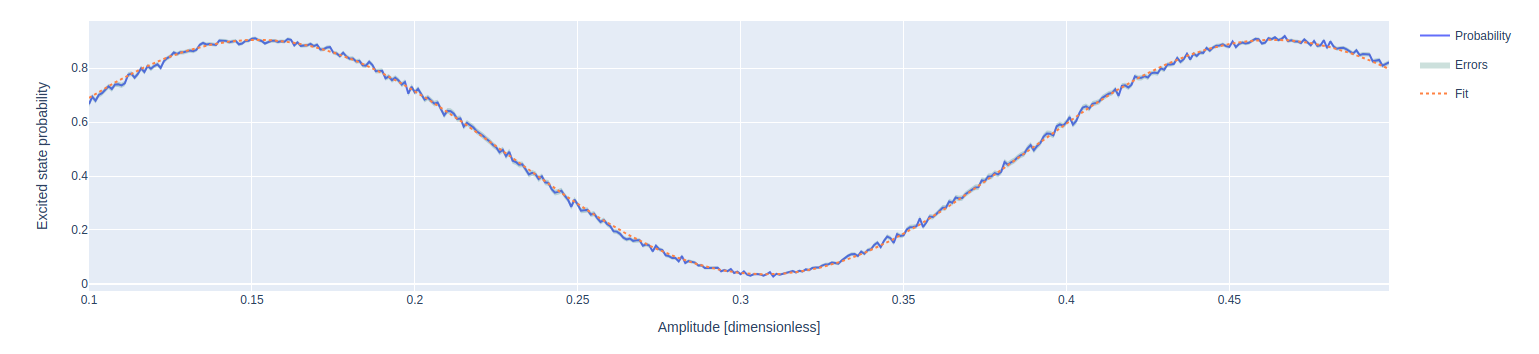
\includegraphics[width=\textwidth]{figures/png/RX90/RabiAmplitude/B4.png}
        \caption{Output of the \tt{rabi\_amplitude} protocol to calibrate the $R_X(\pi)$ gate for qubit \tt{B4}.}
        \label{fig:B4}
    \end{subfigure}
    \vspace{0.3cm}
    \begin{subfigure}[t]{\textwidth}
        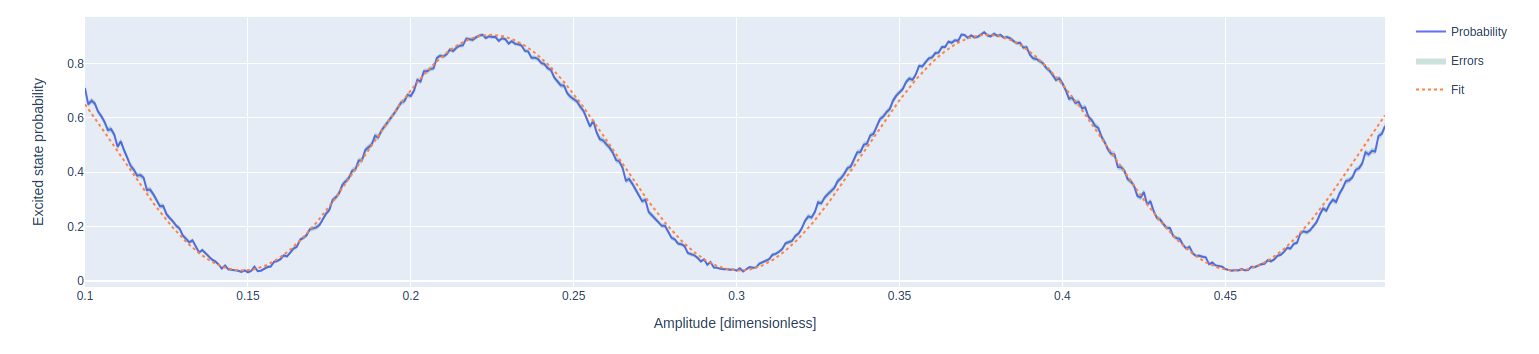
\includegraphics[width=\textwidth]{figures/png/RX90/RabiAmplitude/B4_90.png}
        \caption{Output of the \tt{rabi\_amplitude} protocol to calibrate the $R_X(\pi/2)$ gate for qubit \tt{B4}.}
        \label{fig:B4_90}
    \end{subfigure}
    \caption{Comparison between the results of the amplitude calibration for the $R_X(\pi)$ and $R_X(\pi/2)$ gates.}
    \label{fig:amplitude_comparison}
\end{figure}

\subsubsection{Rabi length}
The pulse duration measurements for the $R_X(\pi)$ and $R_X(\pi/2)$ gates were carried out on the Soprano-D chip by QuantWare \cite{qw5q}, when necessary I will refer to this chip as \tt{qw5q}.
The reason for this is that these measurements were performed after the scheduled cryostat maintenance, and at the time \tt{qw11q} was not yet calibrated.

The sequence of measurements mirrored that used for the amplitude calibration: $R_X(\pi)$ was calibrated first, followed by $R_X(\pi/2)$, with all experimental settings kept fixed except for the \tt{rx90} flag.
An example of the output of the calibration protocol for pulse duration, for both the $R_X(\pi)$ and $R_X(\pi/2)$ gates, is shown in Figures \ref{fig:3} and \ref{fig:3_90}. 

A summary of the quantitative results obtained from these calibrations is presented in Table \ref{tab:length}.
Again, both the inferred value (obtained by halving the $R_X(\pi)$ duration) and the directly calibrated value for the $R_X(\pi/2)$ gate are shown.\\
As in the case of the amplitude calibrations, the standardized difference values are generally positive, indicating that the duration obtained by halving the calibrated $R_X(\pi)$ value tends to be higher than the value obtained from the direct $R_X(\pi/2)$ calibration. 
The only exception to this trend occurs for qubit \tt{5}, for which the standardized difference is negative.
However, unlike the amplitude results discussed previously, the absolute values of the standardized difference are closer to unity or below, suggesting that the discrepancy between the two methods is less pronounced.
This reduction in $|Z|$ can be attributed to two factors: first the smaller absolute difference between the duration values obtained via direct and indirect calibration, and second the larger relative uncertainties associated with the duration estimates compared to those for amplitude.

These observations indicate a more consistent agreement between direct and indirect duration calibrations, although non-negligible deviations still exist and may need further investigation, particularly in the context of high-fidelity gate execution.

\begin{figure}[h!]
    \centering
    \begin{subfigure}[t]{\textwidth}
        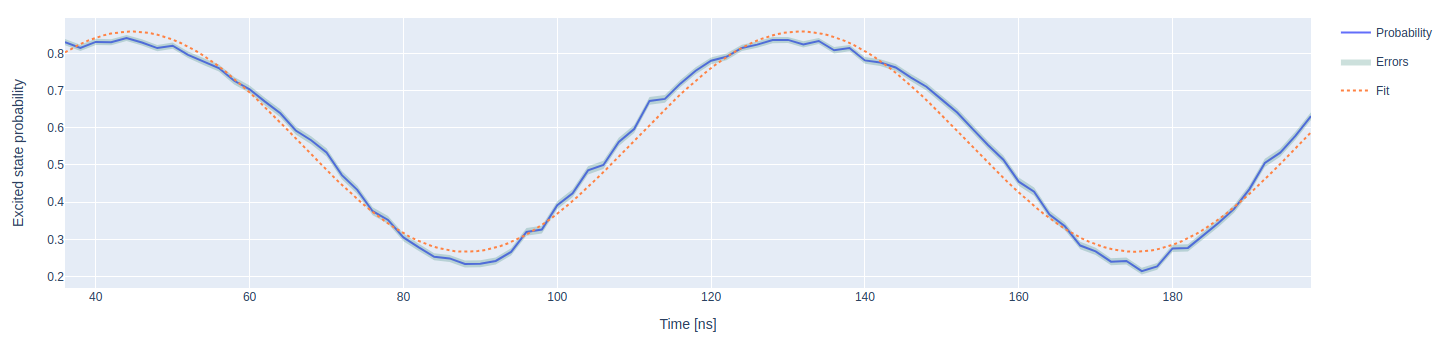
\includegraphics[width=\textwidth]{figures/png/RX90/RabiLength/3.png}
        \caption{Output of the \tt{rabi\_length} protocol to calibrate the $R_X(\pi)$ gate for qubit \tt{3}.}
        \label{fig:3}
    \end{subfigure}
    \vspace{0.3cm}
    \begin{subfigure}[t]{\textwidth}
        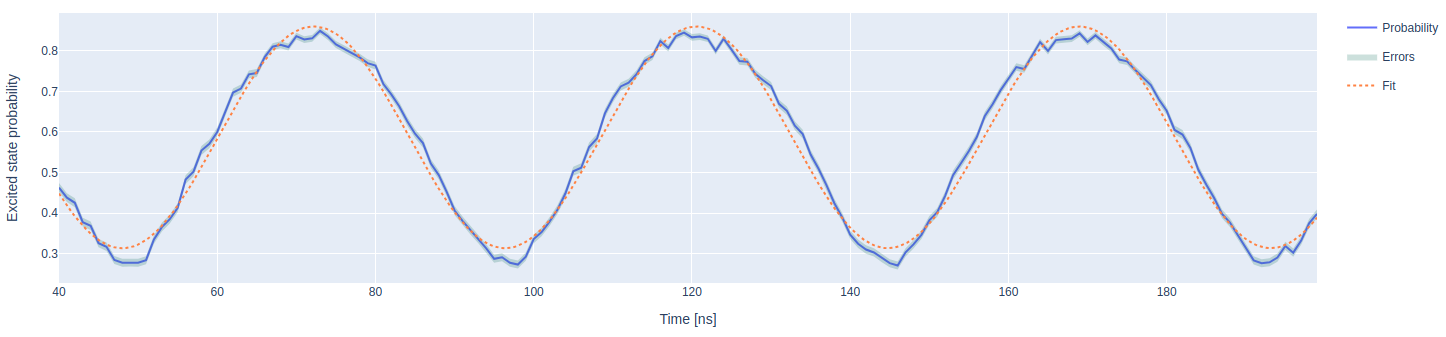
\includegraphics[width=\textwidth]{figures/png/RX90/RabiLength/3_90.png}
        \caption{Output of the \tt{rabi\_length} protocol to calibrate the $R_X(\pi/2)$ gate for qubit \tt{3}.}
        \label{fig:3_90}
    \end{subfigure}
    \caption{Comparison between the results of the duration calibration for the $R_X(\pi)$ and $R_X(\pi/2)$ gates.}
    \label{fig:duration_comparison}
\end{figure}

\subsubsection{Rabi amplitude frequency}
In Figure \ref{fig:af_comparison} I show the results of the Rabi amplitude-frequency calibration experiments, which aim to determine the correct amplitude and frequency for either the $R_X(\pi)$ or $R_X(\pi/2)$ gate, with a fixed pulse duration of 40 ns.
As in previous cases, the scan ranges for amplitude and frequency were held constant between the two experiments; the only difference was the target gate for calibration.

\begin{figure}[h!]
    \centering
    \begin{subfigure}[t]{\textwidth}
        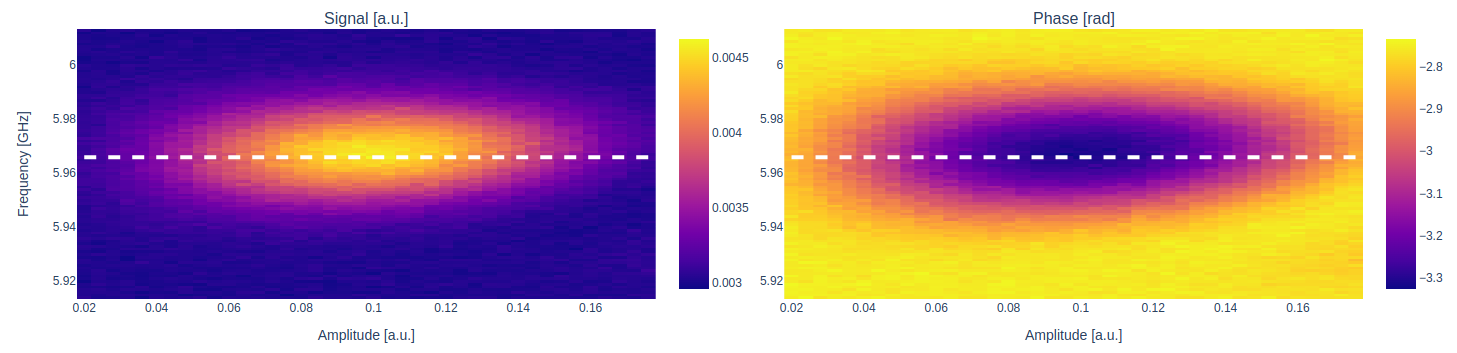
\includegraphics[width=\textwidth]{figures/png/RX90/RabiAmplitudeFrequency/B2.png}
        \caption{Output of the \tt{rabi\_amplitude\_frequency\_signal} protocol to calibrate the $R_X(\pi)$ gate for qubit \tt{B2}.}
        \label{fig:B2}
    \end{subfigure}
    \vspace{0.3cm}
    \begin{subfigure}[t]{\textwidth}
        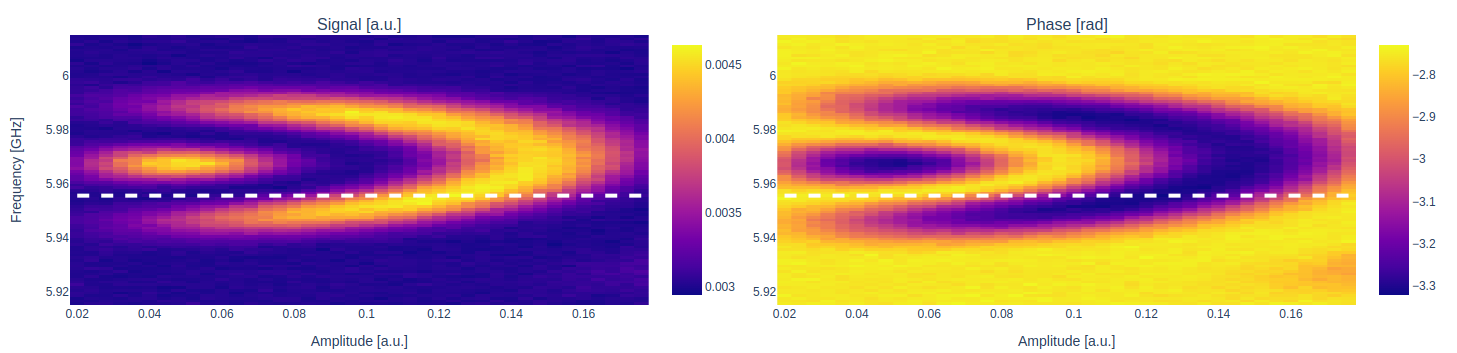
\includegraphics[width=\textwidth]{figures/png/RX90/RabiAmplitudeFrequency/B2_90.png}
        \caption{Output of the \tt{rabi\_amplitude\_frequency\_signal} protocol to calibrate the $R_X(\pi/2)$ gate for qubit \tt{B2}.}
        \label{fig:B2_90}
    \end{subfigure}
    \caption{Comparison between the results of the amplitude and frequency calibration for the $R_X(\pi)$ and $R_X(\pi/2)$ gates.}
    \label{fig:af_comparison}
\end{figure}

Typically, in such experiments, one observes a single peak corresponding to the maximum probability of the qubit being in the excited state $\ket{1}$. 
However, when we extend the scan ranges or, as in this case, we use the same scan intervals for a gate that ideally requires roughly half the amplitude and frequency, the resulting pattern deviates from the usual single-peak expectation. 
Instead, we observe a more complex structure, consistent with the model described by Equation \ref{eq:P1_rabi}.
The ideal interference pattern for the system is shown in Figure \ref{fig:expected_RX90}. 
The amplitude and frequency values used for the plot in Figure \ref{fig:expected_RX90} are not in scale with the real system.

\begin{figure}[h!]
    \centering
    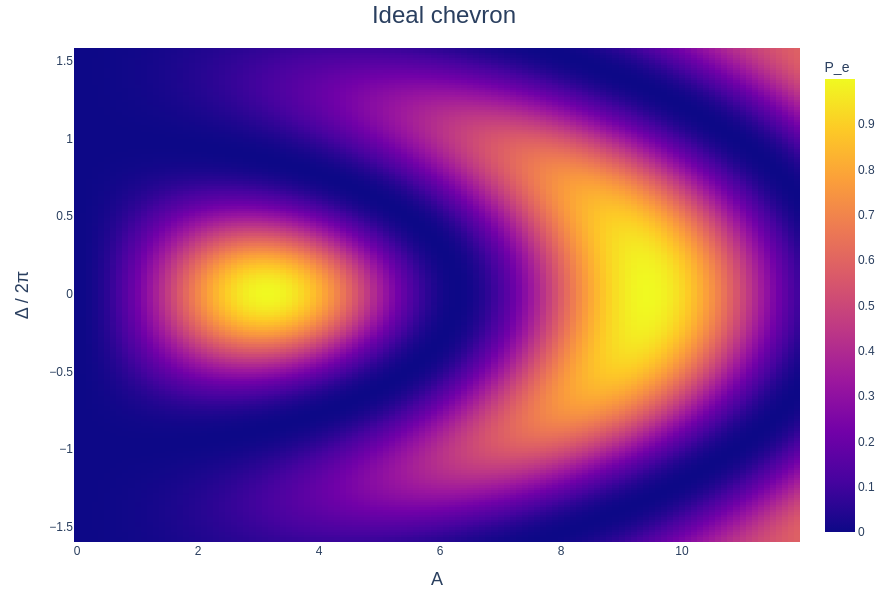
\includegraphics[width=0.495\textwidth]{figures/png/IdealRX90.png}
    \caption{Ideal Rabi oscillation pattern for single qubit varying amplitude and frequency.}
    \label{fig:expected_RX90}
\end{figure}

The figures discussed here are primarily useful from a qualitative standpoint. 
They illustrate how, within the previously effective amplitude and frequency ranges, where a single interference peak was typically observed, we now observe a more complex interference pattern.
However, with such an interference pattern, the standard peak detection algorithm fails to correctly identify the first peak, as we can understand from the misalignment of the dashed line in Figure \ref{fig:B2_90}. 

To allow for a quantitative comparison between the $R_X(\pi/2)$ amplitude obtained through direct calibration and the value inferred from the $R_X(\pi)$ calibration, additional measurements were carried out using modified scan ranges for amplitude and frequency.
For the calibration of the $R_X(\pi)$ gate, the frequency was scanned over a 60 MHz range centered around the qubit frequency, with a step size of 1 MHz. 
The amplitude was scanned in the interval from $0.15$ to $0.35$ with a step of $0.001$.\\
For the calibration of the $R_X(\pi/)$ gate, the frequency was scanned over a 30 MHz range centered around the qubit frequency, with a step size of 1 MHz. 
The amplitude was scanned in the interval from $0.04$ to $0.16$ using a step of $0.01$.\\
The results of these measurements are summarized in Table \ref{tab:af}, and an example of the corresponding interference patterns is shown in Figure \ref{fig:af_qw5q}.

As in the previous cases, the standardized difference values are consistently positive, reflecting that the amplitude obtained by halving the value calibrated for the $R_X(\pi)$ gate is always, even though slightly, greater than the one obtained through a direct calibration of the $R_X(\pi/2)$ gate.
However, n Table \ref{tab:af} it is worth noting that, unlike the results from the other calibration protocols, the magnitude of the standardized difference in this case is consistently less than one. 
This indicates a reasonable agreement between the two estimation methods when experimental uncertainty is taken into account.

It is important to emphasize, however, that this apparent agreement is largely a consequence of the large measurement uncertainty associated with the amplitude values (the average relative error is of the order of $80\%$).

\begin{figure}[h!]
    \centering
    \begin{subfigure}[t]{0.495\textwidth}
        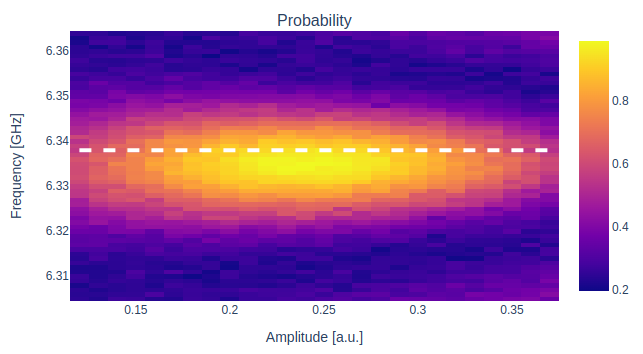
\includegraphics[width=\textwidth]{figures/png/RX90/RabiAmplitudeFrequency/RX.png}
        \caption{Output of the \tt{rabi\_amplitude\_frequency} protocol to calibrate the $R_X(\pi)$ gate for qubit \tt{3}.}
        \label{fig:RX_3}
    \end{subfigure}
    \hfill
    \begin{subfigure}[t]{0.495\textwidth}
        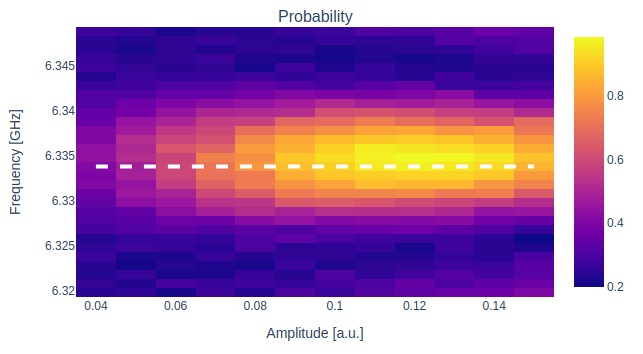
\includegraphics[width=\textwidth]{figures/png/RX90/RabiAmplitudeFrequency/RX90.png}
        \caption{Output of the \tt{rabi\_amplitude\_frequency} protocol to calibrate the $R_X(\pi/2)$ gate for qubit \tt{3}.}
        \label{fig:RX90_30}
    \end{subfigure}
    \caption{Comparison between the results of the amplitude and frequency calibration for the $R_X(\pi)$ and $R_X(\pi/2)$ gates.}
    \label{fig:af_qw5q}
\end{figure}

In Figure \ref{fig:RXvsRX90} I show three plots, each comparing the pulse parameters obtained for implementing an $R_X(\pi/2)$ gate using different calibration strategies, across the various qubits for which the $RX90$ calibration was performed.

An interesting observation, previously mentioned but made more evident when examining the plots, is that both the amplitude and duration estimates for the $R_X(\pi/2)$ gate when obtained by halving the corresponding values calibrated for the $R_X(\pi)$ gate, tend to be slightly overestimated compared to those obtained via direct calibration of the $R_X(\pi/2)$ gate.
This discrepancy is particularly evident for measurements conducted on the \tt{qw11q} chip, as also confirmed by the values of the standardized difference reported in Table \ref{tab:amplitude}.
In contrast, for the \tt{qw5q} chip, the disagreement is noticeably smaller; in particular he standardized difference for amplitude values obtained via the \tt{rabi\_amplitude\_frequency} routine remains below unity in absolute value.
Nevertheless, it is important to emphasize that these latter amplitude values are also associated with larger relative uncertainties and were obtained using a routine that is not the standard one for precise amplitude calibration, but rather intended to provide a rough estimate of the parameter region to explore.

Overall, these results suggest that when circuit execution involves native $R_X(\pi/2)$ gates it may be advantageous to perform a dedicated calibration of the $R_X(\pi/2)$ gate, rather than relying solely on indirect estimates derived from $R_X(\pi)$ gate calibrations. 
This is especially true in scenarios where high gate fidelity is critical or when hardware-specific nonlinearities cannot be neglected.

\begin{figure}[h!]
    \centering
    \begin{subfigure}[t]{0.3\textwidth}
        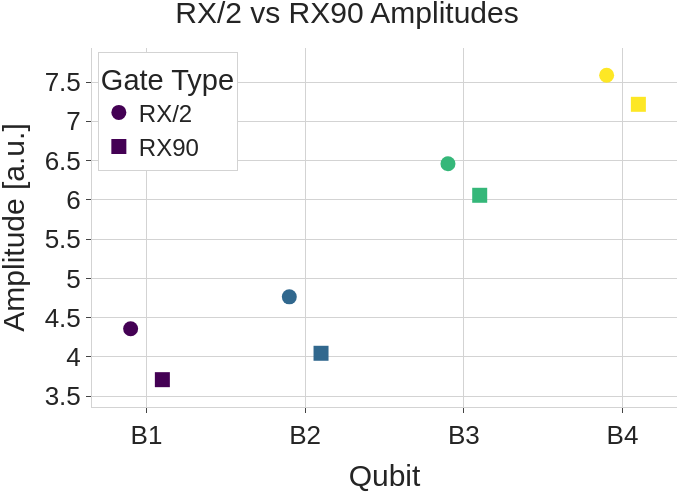
\includegraphics[width=\textwidth]{figures/png/RX90/rabi_amplitude.png}
        \caption{Amplitude of the pulse for the $R_X(\pi/2)$ for different qubits obtained by halving the $R_X(\pi)$ amplitude (circle) or by calibrating the $R_X(\pi/2)$ gate with the \tt{rabi\_amplitude} protocol.}
        \label{fig:RX90_amplitude}
    \end{subfigure}
    \hfill
    \begin{subfigure}[t]{0.3\textwidth}
        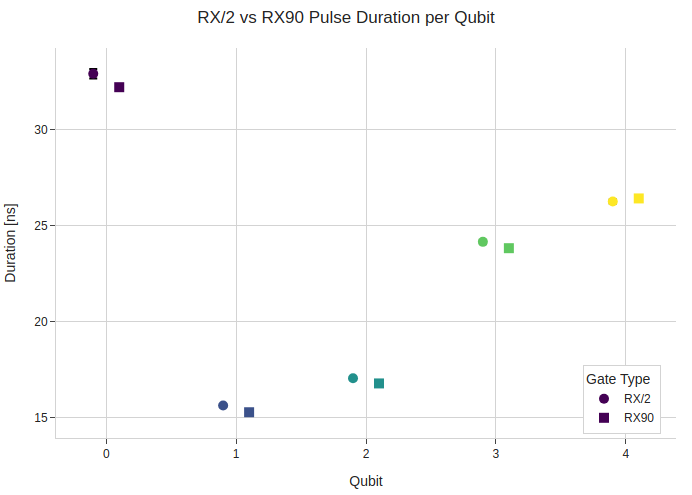
\includegraphics[width=\textwidth]{figures/png/RX90/rabi_length.png}
        \caption{Duration of the pulse for the $R_X(\pi/2)$ for different qubits obtained by halving the $R_X(\pi)$ amplitude (circle) or by calibrating the $R_X(\pi/2)$ gate with the \tt{rabi\_length} protocol.}
        \label{fig:RX90_duration}
    \end{subfigure}
    \hfill
    \begin{subfigure}[t]{0.3\textwidth}
        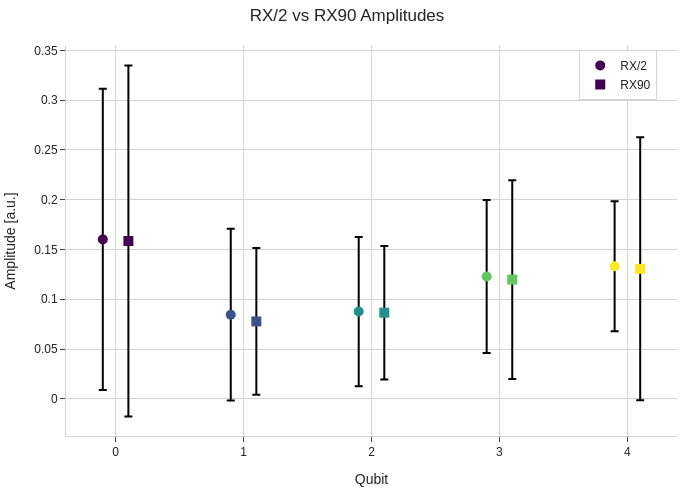
\includegraphics[width=\textwidth]{figures/png/RX90/rabi_af.png}
        \caption{Amplitude of the pulse for the $R_X(\pi/2)$ for different qubits obtained by halving the $R_X(\pi)$ amplitude (circle) or by calibrating the $R_X(\pi/2)$ gate with the \tt{rabi\_amplitude\_frequency} protocol.}
        \label{fig:RX90_af}
    \end{subfigure}
    \caption{The plots show the amplitude (duration) values of the $R_X{\pi/2}$ gate for different qubits obtained from direct calibration or from the calibration of the $R_X(\pi)$ gate.} 
    \label{fig:RXvsRX90}
\end{figure}

Considering both these results and the fact that we wanted to avoid introducing breaking changes to the library, we decided not to replace the $R_X(\pi)$ gate with the $R_X(\pi/2)$ gate as the native gate. Instead, we opted to simply add the $R_X(\pi/2)$ gate to the set of native gates in \Qibolab.

\newpage
\newgeometry{a4paper, top=2.5cm, bottom=2.5cm, inner=1.5cm, outer=1.5cm, heightrounded, bindingoffset=1 cm}

\begin{table}[h!]
    \centering
    \begin{tabular}{c|cc|cc|cc|c}
        \toprule
         & \multicolumn{2}{c|}{\textbf{RX}} & \multicolumn{2}{c|}{\textbf{RX / 2}} & \multicolumn{2}{c|}{\textbf{RX90}} & \textbf{} \\
        \textbf{Qubit} & \textbf{Amplitude} & \textbf{Errors} & \textbf{Amplitude} & \textbf{Errors} & \textbf{Amplitude} & \textbf{Errors} & \textbf{Standardized} \\
         & \textbf{$10^{-2}$[a.u.]} & \textbf{$10^{-2}$[a.u.]} & \textbf{$10^{-2}$[a.u.]} & \textbf{$10^{-2}$[a.u.]} & \textbf{$10^{-2}$[a.u.]} & \textbf{$10^{-2}$[a.u.]} & \textbf{Difference}\\
        \midrule
        \textbf{B1} & 8.72   & 0.001 & 4.36   & 0.005 & 3.711  & 0.006 & 83.095\\
        \textbf{B2} & 9.433  & 0.008 & 4.765  & 0.004 & 4.047  & 0.004 & 126.926\\
        \textbf{B3} & 12.92  & 0.1   & 6.46   & 0.003 & 6.058  & 0.005 & 68.942\\
        \textbf{B4} & 15.17  & 0.1   & 7.585  & 0.005 & 7.216  & 0.005 & 52.184\\
        \bottomrule
    \end{tabular}
    \caption{Amplitude values for the $R_X(\pi)$, half $R_X(\pi)$ and $R_X(\pi/2)$ pulses as measured with the \tt{rabi\_amplitude} protocol with a fixed duration of 40 ns.}
    \label{tab:amplitude}
\end{table}

\begin{table}[h!]
    \centering
    \begin{tabular}{c|cc|cc|cc|c}
        \toprule
         & \multicolumn{2}{c|}{\textbf{RX}} & \multicolumn{2}{c|}{\textbf{RX / 2}} & \multicolumn{2}{c|}{\textbf{RX90}} & \textbf{} \\
        \textbf{Qubit} & \textbf{Duration} & \textbf{Errors} & \textbf{Duration} & \textbf{Errors} & \textbf{Duration} & \textbf{Duration} & \textbf{Standardized} \\
         & \textbf{[ns]}  & \textbf{[ns]}  & \textbf{[ns]}  & \textbf{[ns]} & \textbf{[ns]} & \textbf{[ns]} & \textbf{Difference} \\
        \midrule
        \textbf{0} & 65.8 & 0.5 & 32.9 & 0.25 & 32.2 & 0.1 & 2.599 \\
        \textbf{1} & 31.26 & 0.09 & 15.63 & 0.045 & 15.28 & 0.02 & 7.107\\
        \textbf{2} & 32.1 & 0.07 & 17.05 & 0.035 & 16.78 & 0.02 & 6.698\\
        \textbf{3} & 48.3 & 0.2 & 24.15 & 0.1 & 23.82 & 0.05 & 2.952 \\
        \textbf{4} & 52.5 & 0.3 & 26.25 & 0.1 & 26.41 & 0.06 & -1.372\\
    \end{tabular}
    \caption{Duration values for the $R_X(\pi)$, half $R_X(\pi)$ and $R_X(\pi/2)$ pulses as measured with the \tt{rabi\_length} protocol with a fixed amplitude of 0.2.}
    \label{tab:length}
\end{table}

\begin{table}[h!]
    \centering
    \begin{tabular}{c|cc|cc|cc|c}
        \toprule
         & \multicolumn{2}{c|}{\textbf{RX}} & \multicolumn{2}{c|}{\textbf{RX / 2}} & \multicolumn{2}{c|}{\textbf{RX90}} & \textbf{} \\
        \textbf{Qubit} & \textbf{Amplitude} & \textbf{Errors} & \textbf{Amplitude} & \textbf{Errors} & \textbf{Amplitude} & \textbf{Errors} & \textbf{Standardized} \\
         & \textbf{[a.u.]} & \textbf{[a.u.]} & \textbf{[a.u.]} & \textbf{[a.u.]} & \textbf{[a.u.]} & \textbf{[a.u.]} & \textbf{Difference}\\
        \midrule
        \textbf{0} & 0.3202 & 0.3028 & 0.1601 & 0.1514 & 0.1585 & 0.1763 & 0.007\\
        \textbf{1} & 0.1683 & 0.1725 & 0.08445 & 0.08625 & 0.0777 & 0.0737 & 0.059\\
        \textbf{2} & 0.1752 & 0.1438 & 0.0876 & 0.0749 & 0.0865 & 0.0671 & 0.011\\
        \textbf{3} & 0.2457 & 0.1536 & 0.12285 & 0.0768 & 0.1197 & 0.0998 & 0.025\\
        \textbf{4} & 0.2662 & 0.1305 & 0.1331 & 0.06525 & 0.1305 & 0.1321 & 0.017\\
        \bottomrule
    \end{tabular}
    \caption{Amplitude values for the $R_X(\pi)$, half $R_X(\pi)$ and $R_X(\pi/2)$ pulses as measured with the \tt{rabi\_amplitude\_frequency} protocol with a fixed duration of 40 ns.}
    \label{tab:af}
\end{table}

\newpage
\restoregeometry
\section{Flux pulse correction}

\subsection{Cryoscope}
The protocol that I describe in this section was first introduced in \cite{rol_time-domain_2020}, the goal is to reconstruct the magnetic flux signal that biases the SQUID and then determine predistortions that need to be applied so that the qubit receives the flux pulse as intended by the experimenter.

As explained in section \ref{sec:cQED}, accurate dynamical control of qubit frequency is of key importance to realize single- and two-qubit gates.
One of the on-chip control variables that is used on the QunatumWare chip is the magnetic flux through a SQUID loop, the signal for magnetic flux control originates from an arbitrary waveform generator (AWG) which operates at room temperature.\\
As the signal propagates through various electrical components along the control line leading to the chip it undergoes linear dynamical distortions. 
If not properly compensated, these distortions can degrade gate performance, impacting experiment fidelity and repeatability.\\

In \cite{rol_time-domain_2020} is proposed a technique to characterize flux-pulse distortions induced by components inside the dilution refrigerator by directly measuring the qubit state.
In this routine, we send the qubit a pulse sequence where a flux pulse of varying duration $\tau$ is embedded between two $\frac{\pi}{2}$ pulses which are always separated by a fixed interval $T_{sep}$.\\
The first $\frac{\pi}{2}$ pulse rotates the qubit of $\frac{\pi}{2}$ around the $y$ axis of the Bloch sphere changing its state from $\ket{0}$ to $\frac{\ket{0}+\ket{1}}{\sqrt{2}}$.

When a flux pulse $\Phi_{Q,\tau}(t)$ of duration $\tau$ is sent to the qubit\footnote{To send a $\Phi_{Q,\tau}(t)$ flux pulse we are actually sending a $V_{\text{in},\tau}(t)$ DAC pulse} after the first $\frac{\pi}{2}$ pulse, the qubits evolve to the state $\frac{\ket{0}+e^{i\varphi_\tau}\ket{1}}{\sqrt{2}}$ with relative quantum phase 
\begin{equation}\label{eq:phi}
    \frac{\varphi_{\tau}}{2\pi} = \int_{0}^{T_{sep}} \Delta f_Q (\Phi_{Q,\tau(t)})\text{d}t = \int_{0}^{\tau} \Delta f_Q (\Phi_{Q,\tau(t)})\text{d}t + \int_{\tau}^{T_{sep}} \Delta f_Q (\Phi_{Q,\tau(t)})\text{d}t
\end{equation}
where in the second step I separated the contributions from flux response up to $\tau$ and the turn-off transient \footnote{In Appendix \ref{app:phase_rec} we calculate the relative phase $\varphi_{\tau}$ for a more general shape of the flux pulse.}. 

The experiment is then completed with a $\frac{\pi}{2}$ rotation around the $y$- or $x$-axis of the Bloch sphere to measure respectively the $\langle X \rangle$ or $\langle Y \rangle$ components of the Bloch vector when applying the measurement gate $MZ$. 
From the measurement of $\langle X \rangle$ and $\langle Y \rangle$ we can extract the relative phase $\varphi_{\tau}$.
For detailed calculations on how $\langle X \rangle$ and $\langle Y \rangle$ are measured and $\varphi_{\tau}$ extracted see Appendix \ref{app:XY_measure}. \\ 

Then we can estimate $\Phi_Q(t)$ in the interval $[\tau,\tau+\Delta\tau]$ as follows. From the measurement of $\varphi_{\tau + \Delta\tau}$ and $\varphi_\tau$ we can compute $\overline{\Delta f_R}$:
\begin{align}\label{eq:detuning}
    \overline{\Delta f_R} &= \frac{\varphi_{\tau+\Delta\tau} - \varphi_\tau}{2\pi\Delta\tau}\\ 
    &= \frac{1}{\Delta\tau}\left(\int_{0}^{\tau+\Delta\tau}\Delta f_Q (\Phi_{Q,\tau+\Delta\tau}(t))dt + \int_{\tau+\Delta\tau}^{T_{sep}}\Delta f_Q (\Phi_{Q,\tau+\Delta\tau}(t))dt\right) \\
    &-\frac{1}{\Delta\tau}\left(\int_{0}^{\tau}\Delta f_Q (\Phi_{Q,\tau}(t))dt - \int_{\tau}^{T_{sep}}\Delta f_Q (\Phi_{Q,\tau}(t))dt\right)\\
    &=\frac{1}{\Delta\tau}\left(\int_{\tau}^{\tau+\Delta\tau} \Delta f_Q(\Phi_{Q,\tau+\Delta\tau})dt + \int_{\tau+\Delta\tau}^{T_{sep}}\Delta f_Q (\Phi_{Q,\tau+\Delta\tau}(t))dt - \int_{\tau}^{T_{sep}}\Delta f_Q (\Phi_{Q,\tau}(t))dt\right)\\
    &= \frac{1}{\Delta\tau}\int_{\tau}^{\tau+\Delta\tau} \Delta f_Q(\Phi_{Q,\tau+\Delta\tau})dt + \varepsilon
\end{align}  
with \[\varepsilon = \frac{1}{\Delta\tau}\left(\int_{\tau+\Delta\tau}^{T_{sep}}\Delta f_Q (\Phi_{Q,\tau+\Delta\tau}(t))dt - \int_{\tau}^{T_{sep}}\Delta f_Q (\Phi_{Q,\tau}(t))dt\right)\]
The phase contribution from the turn-off transients is minimal due to the sharp return to the first-order flux-insensitive sweet spot of the nearly quadratic $\Delta f_Q(\Phi_Q)$; 
numerical simulations suggest that $|\varepsilon|/\Delta f_R$ remains within the range of approximately $10^{-2}$ to $10^{-3}$ for typical dynamical distortions in commonly used electronic components \cite{negligible} \cite{Langford2017}, for this reason it will be neglected.\\

At this point, we can obtain the reconstructed flux pulse $\Phi_R(t)$ inverting Equation \ref{eq:freqdepndenceonflux}.

In the following sections I will describe how we used this protocol to reconstruct the voltage-to-flux step response, and then how to determine and apply pre-distortion corrections to the control waveforms.

\subsubsection{Experimental parameters}
The first step in implementing the cryoscope protocol involves building the appropriate pulse sequence. 
As described before, the protocol for reconstructing the flux pulse is a Ramsey-like experiment in which a flux pulse of variable duration $\tau$ is embedded between two microwave $\frac{\pi}{2}$ pulses, separated by a fixed delay $T_{sep}$.

In our implementation, we fixed $T_{sep}$ to $100$ ns longer than the maximum duration of the flux pulse; this approach avoids the need for fine timing calibration, as mentioned also in Rol et al \cite{rol_time-domain_2020}.
The variation in pulse duration $\Delta\tau$ is user-defined and determines the sampling resolution of the time-dependent frequency shift.
Specifically, users configure the experiment via a runcard \footnote{In Qibocal, all protocols are deployed through a YAML-based runcard, which allows the user to specify experiment-specific parameters.}
where they set the minimum (\tt{duration\_min}) and maximum (\tt{duration\_max}) durations of the flux pulse, along with the duration increment (\tt{duration\_step}), which corresponds to the interval $\Delta\tau$ used in Equation \ref{eq:detuning}.
The lower bound $\Delta\tau$ is constrained by the sampling capabilities of the acquisition hardware.
For all data and analyses reported in this section, we used the OPX1000 by Quantum Machines \cite{opx1000} as an acquisition device. 
The OPX1000 has a sampling rate of 1 GSample/s, corresponding to a temporal resolution of $1$ ns which sets a lower limit $\Delta\tau \geq 1$ ns for the acquisition.

The amplitude of the flux pulse, specified by the user through the parameter \tt{flux\_pulse\_amplitude}, can also be configured in the runcard. 
While this parameter is user-defined, it is advisable to select an amplitude that induces a detuning from the qubit's sweet spot comparable to that used in typical flux-pulsed gate operations. 
This ensures that the measured system response is representative of practical use cases.
For example, it is useful to study the qubit response to a flux pulse which induces a frequency detuning of approximately 1 GHz. 
This detuning value is commonly employed in high-fidelity entangling gate implementations \cite{Langford2017}, \cite{Bultink_2020}, \cite{Rol2019iju}.

In the initial analysis conducted to develop the cryoscope routine for the flux pulse, we used a waveform defined as a combination of two-step functions. 
Specifically, the waveform remains at zero for the first $10$ ns, rises to a nominal unit amplitude for the subsequent $50$ ns, and returns to zero for the final $10$ ns.
The flux pulse amplitude used for this first acquisition and the corresponding preliminary analyses was $0.1$, which, as observed using the \tt{flux\_amplitude\_frequency} routine, induces a detuning of approximately $0.01$ GHz in qubit \tt{D1}. 

Given the relatively small detuning, we decided to perform an additional acquisition using a flux pulse with a higher amplitude to obtain more reliable results.
For this second acquisition, a \tt{flux\_pulse\_amplitude} of $0.5$ was used, corresponding to a detuning of approximately $0.5$ GHz. 
In this case, the waveform was also modified: a single step pulse of unit amplitude and $90$ ns duration was applied, with no initial or final padding.

In the following, I will refer to the two waveforms as waveform\_1 and waveform\_2. 
The shapes of both waveforms are shown in Figure \ref{fig:ideal_waveform}

\begin{figure}[h!]
    \centering    
    \begin{subfigure}[t]{0.495\textwidth}
        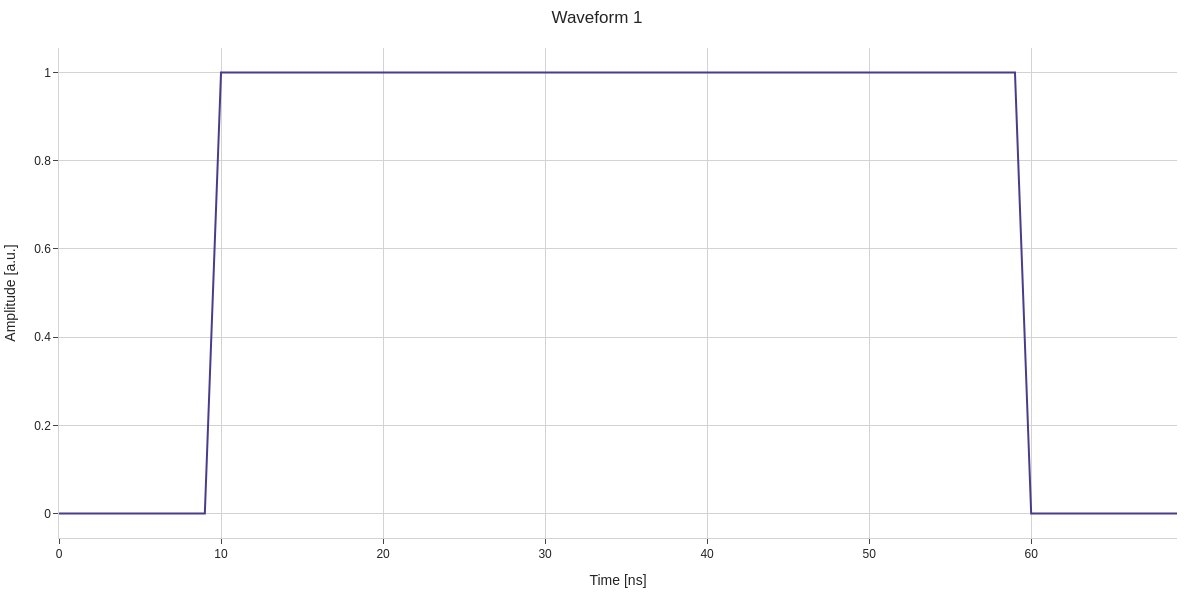
\includegraphics[width=\textwidth]{figures/png/Cryoscope/waveform1.png}
        \caption{Plot of the ideal flux pulse for waveform\_1.}
        \label{fig:waveform1}
    \end{subfigure}
    \hfill
    \begin{subfigure}[t]{0.495\textwidth}
        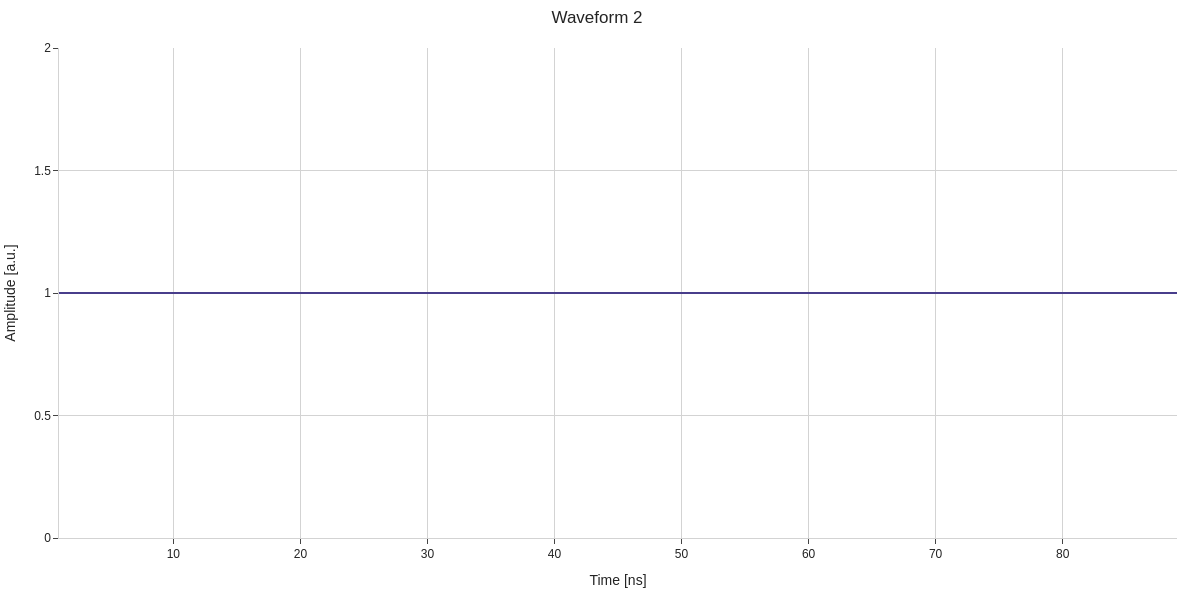
\includegraphics[width=\textwidth]{figures/png/Cryoscope/waveform2.png}
        \caption{Plot of the ideal flux pulse for waveform\_2.}
        \label{fig:waveform2}
    \end{subfigure}

    \caption{Plot of the ideal waveform of the flux pulse.}
    \label{fig:ideal_waveform}
\end{figure}

The decision to perform tests with the second, longer waveform, omitting initial padding, was motivated by practical considerations related to the pulse reconstruction process. 
In particular, since the qubit's response is only affected during periods when a non-zero flux is applied, the system behavior before the pulse onset is less relevant for reconstruction purposes.
Our primary focus is on characterizing the qubit's dynamics during the flux pulse and, potentially, in the transient period following its termination, to assess how long it takes for the qubit to return to its idle frequency after the pulse is switched off
\footnote{Although we did not focus on this aspect, this is relevant in practical applications, as it allows for shorter idle times between pulses and thus enables a higher number of gate operations within a given time window.}.
All experimental results and analyses presented herein are based on data acquired from qubit \tt{D1} of chip \tt{qw11q} unless differently specified.

\subsubsection{Phase reconstruction}
The first step in analyzing the cryoscope data involves isolating the oscillatory components of the signals corresponding to the $\langle X \rangle$ and $\langle Y \rangle$ measurements. 
These oscillations reflect the coherent evolution of the qubit under the influence of the applied flux pulse.

What is experimentally measured for each observable is the probability $p_1(t)$ of finding the qubit in the excited state $\ket{1}$ as a function of time. 
From this probability, we reconstruct the temporal evolution of the $z$-component of the Bloch vector using the relation:
\begin{equation}
z(t) = 1 - p_1(t).
\end{equation}
The reconstructed $z(t)$ signal is then fitted with an exponentially decaying sinusoid, analogous to the fitting procedure used in Ramsey experiments.
This fitting is performed independently on the traces obtained from the $\langle X(t) \rangle$ and $\langle Y(t) \rangle$ measurements, allowing us to estimate the characteristic oscillation frequencies associated with each case.

At this point, to access the phase evolution, we reconstruct the complex signal $s(t) = \langle X(t) \rangle + i\langle Y(t) \rangle$. 
To do this, we use the following relations:
\begin{align}
    & \langle X \rangle = 2p^X_1 - 1 \\
    & \langle Y \rangle = 1 - 2p^Y_1
\end{align}
where $p^X_1(t)$ and $p^Y_1(t)$ denote the measured probabilities of finding the qubit in state $\ket{1}$ from the $\langle X \rangle$ and $\langle Y \rangle$ measurements, respectively.
The derivations of these relations is reported in Appendix \ref{app:XY_measure}.

Once the characteristic oscillation frequency has been estimated, we demodulate the signal by this frequency: $s_{\text{demod}}(t) = e^{2\pi i f_{\text{demod}} t} \cdot s(t)$
This operation shifts the signal's frequency content to near-zero removing the fast oscillations and leaving only the slower variations in phase.

This step is important because the raw signal may oscillate rapidly, making it difficult to directly extract the underlying phase dynamics. 
Demodulation transforms the signal into a smooth, slowly varying function of time, allowing for reliable computation of the phase and its derivative and, in turn, of the instantaneous detuning.
Once demodulated, the time-dependent phase of the signal is extracted from the complex argument of the demodulated data. 
Without this preprocessing, the dominant carrier frequency could overshadow the relevant phase information.

\begin{figure}[h!]
    \centering
    \begin{subfigure}[t]{0.495\textwidth}
        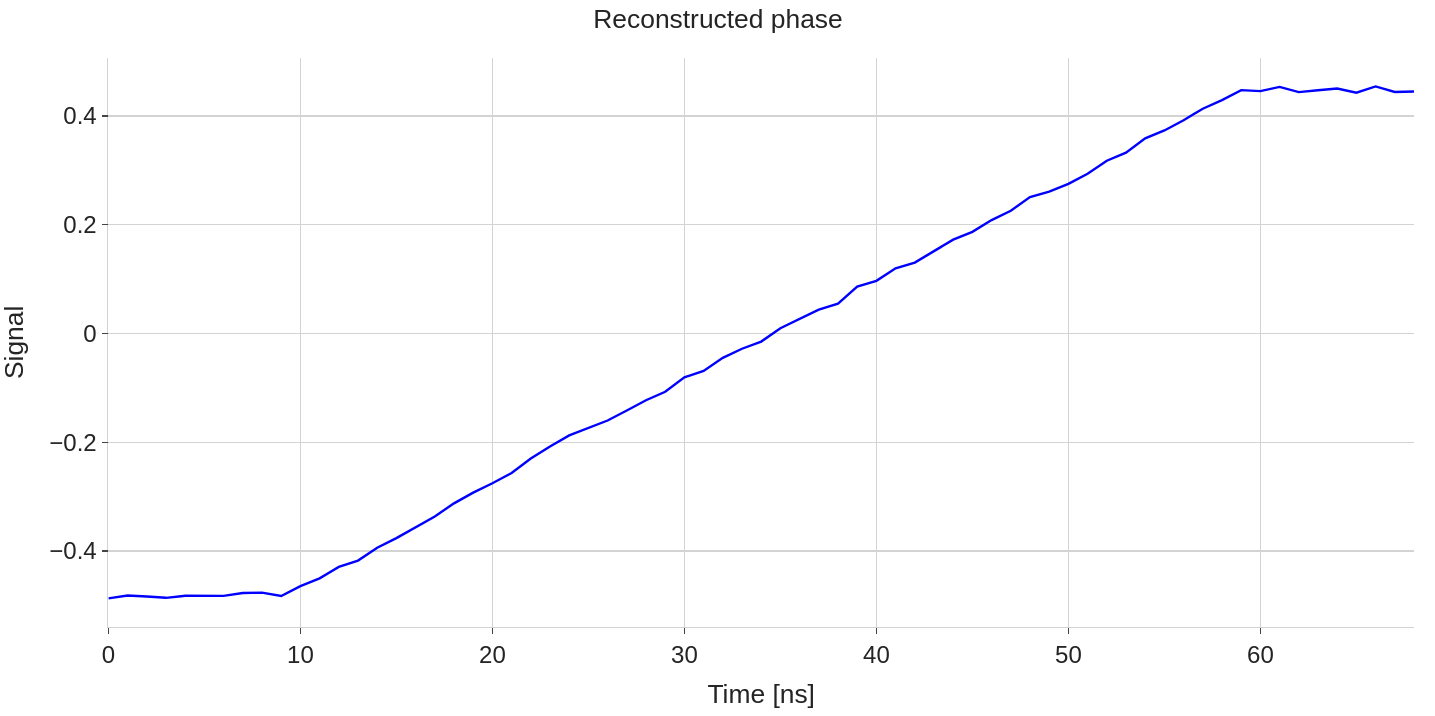
\includegraphics[width=\textwidth]{figures/png/Cryoscope/no_demod/Screenshot From 2025-06-08 12-21-41.png}
        \caption{Reconstruction of the phase evolution of the qubit under a flux pulse of shape waveform\_1 with no demodulation applied on the acquired data.}
        \label{fig:no_demodulation:step}
    \end{subfigure}
    \hfill
    \begin{subfigure}[t]{0.495\textwidth}
        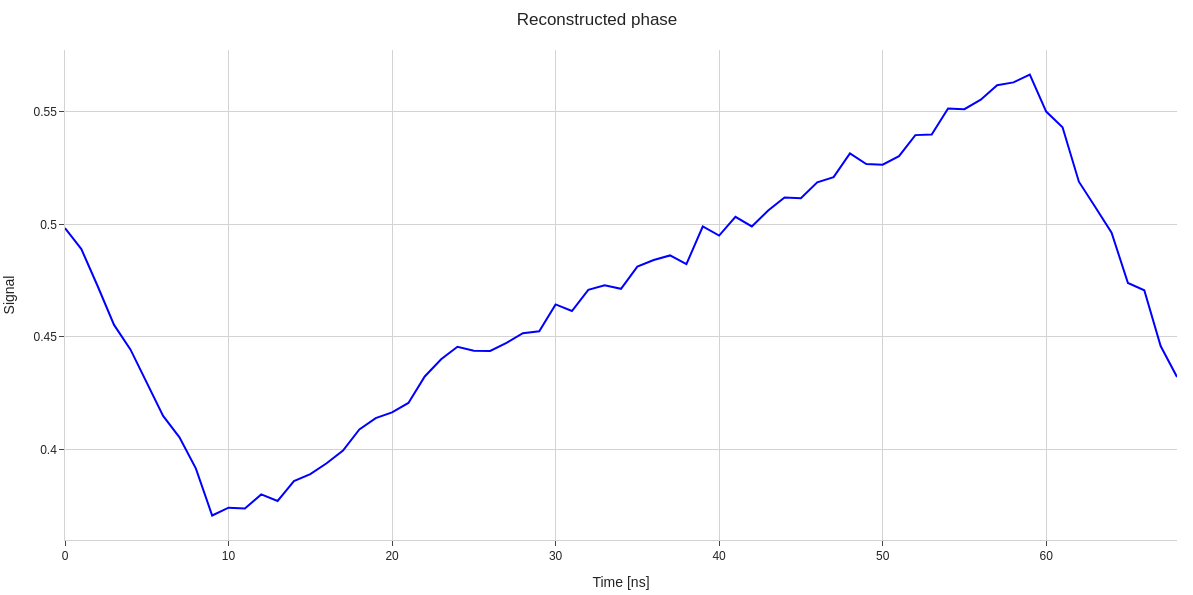
\includegraphics[width=\textwidth]{figures/png/Cryoscope/demodulation/phase.png}
        \caption{Reconstruction of the phase evolution of the qubit under a flux pulse of shape waveform\_1 with demodulation applied on the acquired data.}
        \label{fig:demodulation:step}
    \end{subfigure}

    \vspace{0.5cm}

    \begin{subfigure}[t]{0.495\textwidth}
        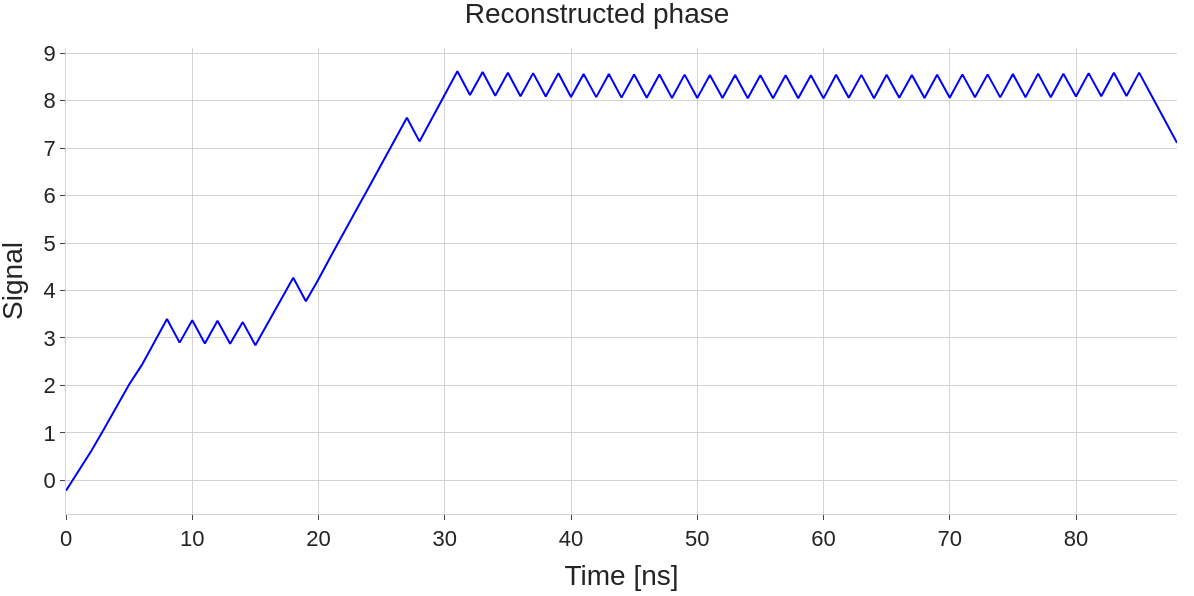
\includegraphics[width=\textwidth]{figures/png/Cryoscope/no_demod/long/phase.png}
        \caption{Reconstruction of the phase evolution of the qubit under a flux pulse of shape waveform\_2 with no demodulation applied on the acquired data.}
        \label{fig:no_demodulation:long}
    \end{subfigure}
    \hfill
    \begin{subfigure}[t]{0.495\textwidth}
        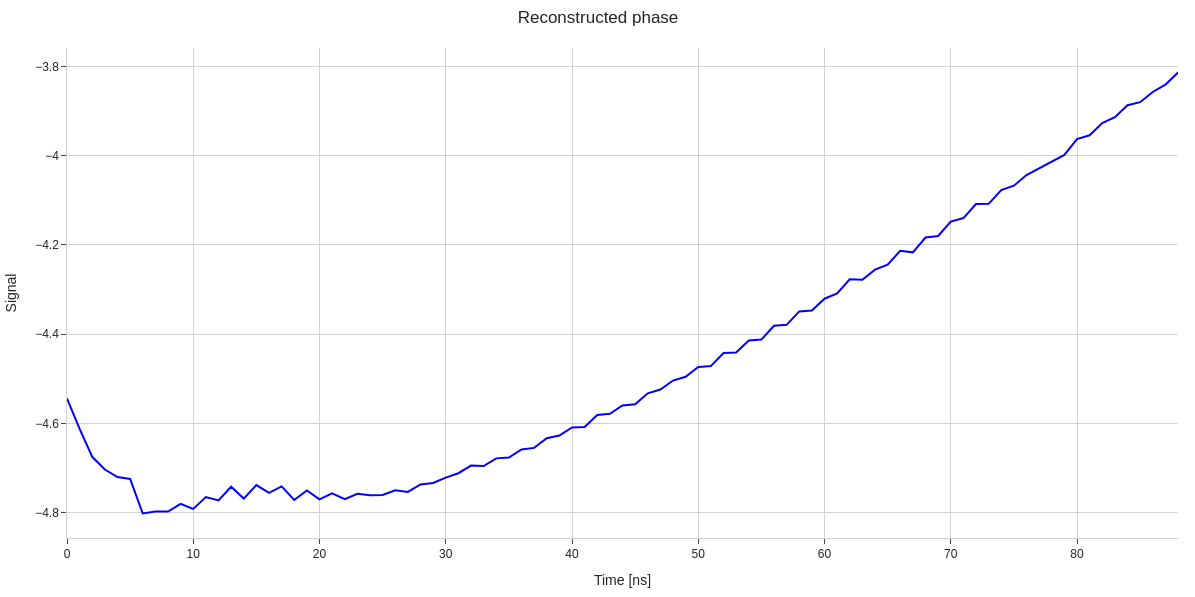
\includegraphics[width=\textwidth]{figures/png/Cryoscope/demodulation/long/phase.png}
        \caption{Reconstruction of the phase evolution of the qubit under a flux pulse of shape waveform\_1 with demodulation applied on the acquired data.}
        \label{fig:demodulation:long}
    \end{subfigure}

    \caption{Examples of reconstruction of the phase evolution of a superconducting qubit under the action of a flux pulse with different waveforms.}
    \label{fig:demodulation}
\end{figure}

By comparing Figure \ref{fig:no_demodulation:step} and Figure \ref{fig:demodulation:step}, the first observation we can make is that the reconstructed qubit phase begins to vary immediately after $t=10$ ns, while remaining essentially constant up to $t=9$ ns. 
This seems to suggest that, at least within this time window, the flux pulse onset and the resulting qubit frequency shift happen quickly, with no evident latency.
One possible explanation for the fast response observed at low flux amplitude $A = 0.1$, is that the flux pulse reaches its nominal value rapidly, making the expected exponential rise in frequency shift too fast to be resolved. 
Additionally, the small amplitude induces a weak detuning, leading to slow phase accumulation that may be more susceptible to background noise, potentially obscuring the signal.

A second observation is that the demodulated signal in Figure \ref{fig:demodulation:step} appears to exhibit increased phase oscillations compared to the non-demodulated case, potentially giving the impression that demodulation degrades the phase signal quality. 
However, a clearer picture emerges when considering the full temporal evolution, as shown in Figures \ref{fig:no_demodulation:long} and \ref{fig:demodulation:long}. 
In the non-demodulated case (Figure \ref{fig:no_demodulation:long}), the reconstructed phase signal is highly oscillatory, making it difficult to identify the qubit evolution. 
In contrast, the demodulated signal in Figure \ref{fig:demodulation:long} yields a much smoother phase trajectory, clearly revealing the onset and development of a frequency shift.

Notably, unlike the seemingly abrupt transition observed in the short time window (Figure \ref{fig:demodulation:step}), the long-timescale demodulated phase shows a gradual evolution, indicating that the flux pulse requires a finite rise time to reach its full amplitude. 
During this transient phase, the qubit frequency, and hence the rate of phase accumulation, increases progressively. 
This behavior is consistent with the physical expectation that the flux pulse ramps up smoothly, and it highlights the importance of demodulation in accurately recovering the continuous phase evolution of the qubit in response to the pulse.

\subsubsection{Flux pulse reconstruction}
After reconstructing the phase signal from the demodulated complex data, we can estimate the instantaneous detuning of the qubit by computing the time derivative of this phase. 
As explained at the beginning of this Section, the rate at which the phase accumulates corresponds to the detuning (see Equation \ref{eq:detuning}). 

\paragraph{Savitzky-Golay filter}
To perform this differentiation in a way that reduces the impact of noise, we used a Savitzky-Golay filter, which operates by fitting a polynomial to small segments of the data along the time axis. In this work, we used the \tt{scipy.signal} implementation of the signal with the default settings where possible. 
In particular, the filter runs in \tt{'interp'} mode, which doesn't pad or extend the signal at the edges; instead, it fits a polynomial to the last few data points and uses that to estimate the values near the boundaries.

For our analysis, we use a polynomial order of 2 and explore how different values of \tt{window\_length} affect the final detuning signal. 
The choice of \tt{window\_length} is particularly important because the Savitzky-Golay filter effectively acts similarly to a moving average. 
This has some relevant consequences. First, if the window is too small, the filter does not average over enough points to effectively suppress high-frequency noise, making the derivative signal noisier. 
On the other hand, if the window is too large, it can over-smooth the signal and distort fast transitions. 
If the window is too large, the filter may incorporate data from the initial flat region into the fit, which can artificially stretch the signal's rising edge or introduce distortions at the boundaries. 
This can give the impression of a slower onset of the phase response than what is physically accurate, and such edge effects are particularly noticeable when the signal includes an initial segment of zero flux.

The effect of different \tt{window\_length} values on the reconstructed detuning is shown in Figure \ref{fig:detuning}.

\begin{figure}[h!]
    \centering
    \begin{subfigure}[t]{0.495\textwidth}
        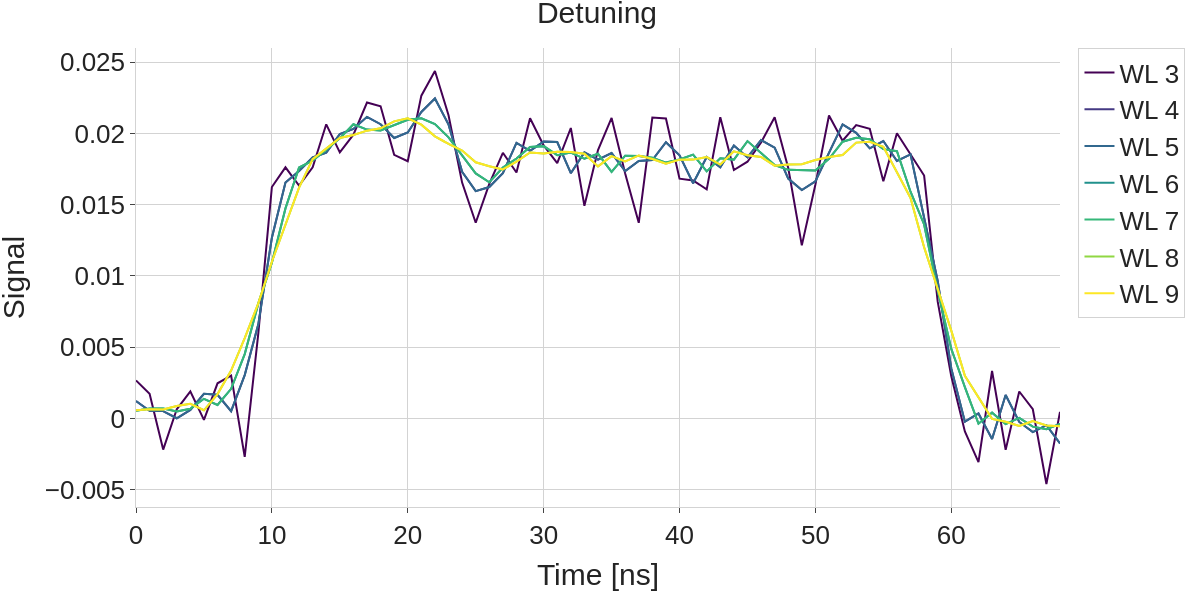
\includegraphics[width=\textwidth]{figures/png/Cryoscope/no_demod/detuning_windows.png}
        \caption{Reconstruction of the detuning of the qubit under a flux pulse of shape waveform\_1 without demodulation applied on the acquired data.}
        \label{fig:detuning:step_no_dem}
    \end{subfigure}
    \hfill
    \begin{subfigure}[t]{0.495\textwidth}
        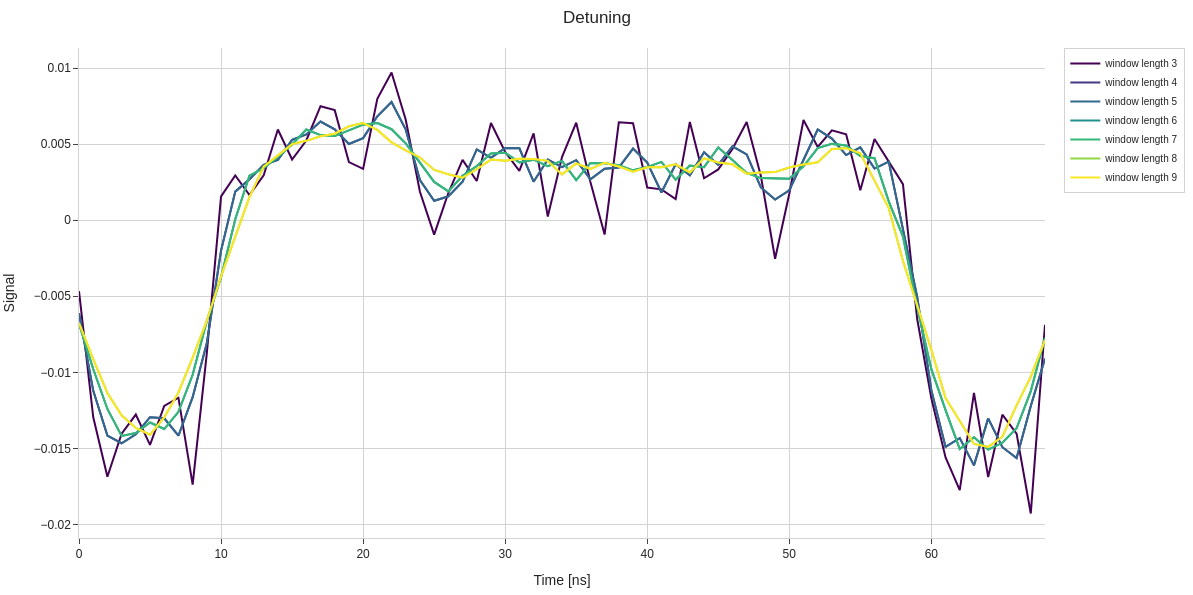
\includegraphics[width=\textwidth]{figures/png/Cryoscope/demodulation/detuning_windows.png}
        \caption{Reconstruction of the detuning of the qubit under a flux pulse of shape waveform\_1 with demodulation applied on the acquired data.}
        \label{fig:detuning:step_dem}
    \end{subfigure}

    \vspace{0.5cm}

    \begin{subfigure}[t]{0.495\textwidth}
        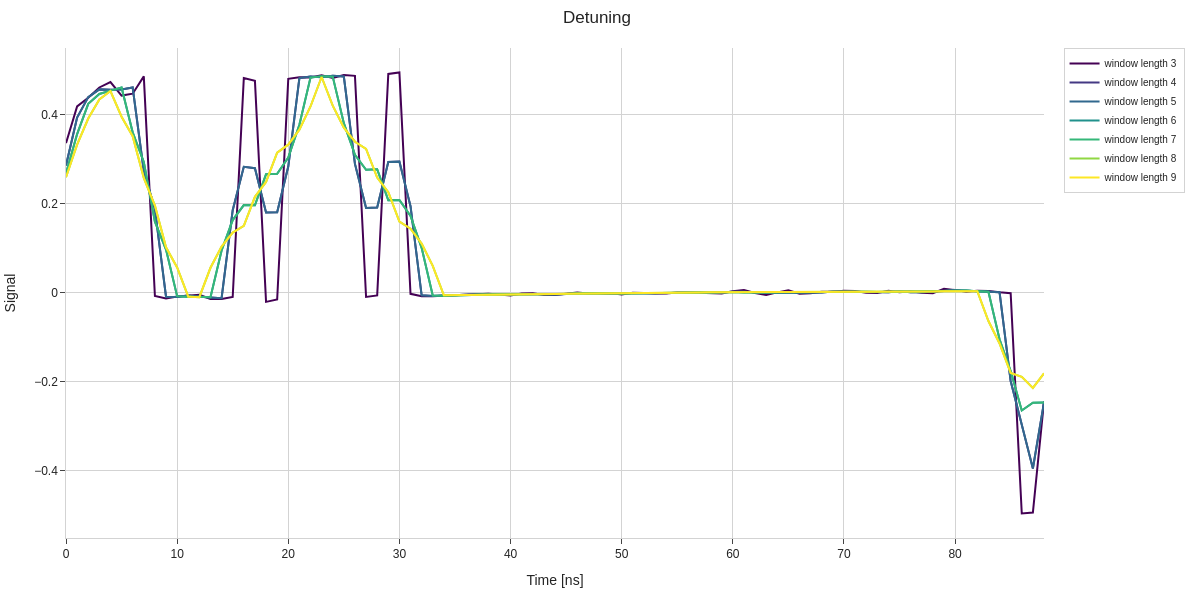
\includegraphics[width=\textwidth]{figures/png/Cryoscope/no_demod/long/detuning_windows.png}
        \caption{Reconstruction of the detuning of the qubit under a flux pulse of shape waveform\_2 without demodulation applied on the acquired data.}
        \label{fig:detuning:long_no_dem}
    \end{subfigure}
    \hfill
    \begin{subfigure}[t]{0.495\textwidth}
        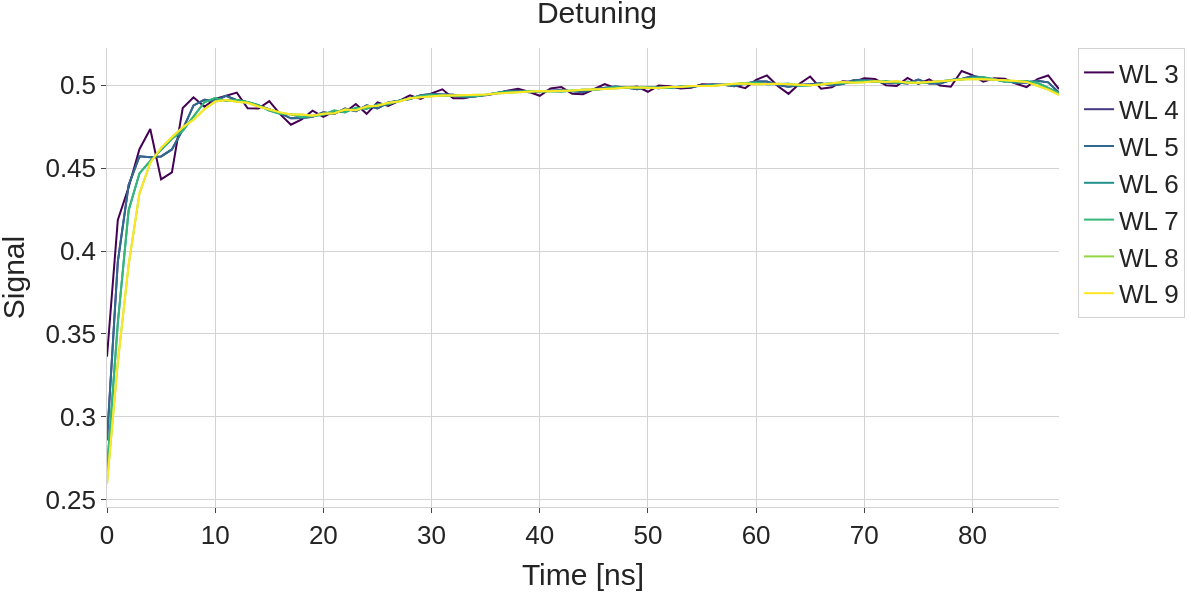
\includegraphics[width=\textwidth]{figures/png/Cryoscope/demodulation/long/detuning_windows.png}
        \caption{Reconstruction of the detuning of the qubit under a flux pulse of shape waveform\_2 with demodulation applied on the acquired data.}
        \label{fig:detuning:long_dem}
    \end{subfigure}

    \caption{Examples of reconstruction of the detuning of a superconducting qubit under the action of a flux pulse with different waveforms.}
    \label{fig:detuning}
\end{figure}

This tuning is especially important because the detuning is obtained by differentiating the phase signal, which amplifies any residual oscillations or imperfections. 
This issue becomes evident in the acquisition performed with \tt{waveform\_1} at an amplitude of $0.1$, where the flux pulse is preceded by $10$ ns of zero signal. 
In this case, two non-physical responses appear in the signal: first, the detuning appears to evolve even before the flux pulse is applied, giving the impression of a non-causal response; second, an exponential rise is observed in the reconstructed detuning that is not actually present in the qubit phase signal. 
These spurious effects are largely absent when the acquisition window is extended and the signal starts immediately with the pulse, but we nonetheless explored how different values of \tt{window\_length} affect the final result.

In particular, we tested values of \tt{window\_length} corresponding to a range between $3$ and $10$. 
The lower bound of 3 is set by the minimum required for a second-order polynomial fit, as the filter requires that \tt{polyorder} must be less than \tt{window\_length}.

Figure \ref{fig:detuning} shows the reconstructed detuning under different conditions. 
In particular, panels \ref{fig:detuning:step_no_dem} and \ref{fig:detuning:long_no_dem} include results obtained without applying demodulation. 
For the first flux pulse, although demodulation introduces additional oscillations in the phase signal, it does not substantially affect the final detuning.
The main discrepancy appears at the signal boundaries, where the ideally zero detuning, shows sharp, unphysical variations amplified by the effect of differentiation.

The situation is different for the second flux pulse. 
Without demodulation, the detuning reconstruction fails to reflect the expected physical behavior, as seen in Figure \ref{fig:detuning:long_no_dem}. 
In contrast, when demodulation is applied, as shown in Figure \ref{fig:detuning:long_dem}, the reconstructed detuning clearly follows the anticipated pattern: an exponential onset followed by a stable plateau, consistent with a qubit experiencing a constant-amplitude flux pulse.

Finally, after reconstructing the qubit detuning, we invert the relationship between detuning and applied flux amplitude described by equation \ref{eq:freqdepndenceonflux_approx}, to recover the actual flux amplitude as a function of time. 
Specifically, we assume a quadratic model of the form
\begin{equation}
    f = c_1 A^2 + c_2 A + c_3,
\end{equation}
where $f$ denotes the detuning, $A$ is the applied flux amplitude, and $c_1$, $c_2$, and $c_3$ are coefficients obtained from the \tt{flux\_amplitude\_frequency} routine (see Appendix \ref{app:flux_amplitude_frequency} for more details). 
By inverting this relation, we reconstruct the time-dependent flux amplitude experienced by the qubit. 
The results of this reconstruction are shown in Figure \ref{fig:amplitude}.
For completeness, I have included the plots related to the amplitude reconstruction performed for all previously discussed cases, both with and without demodulation.

\begin{figure}[h!]
    \centering
    \begin{subfigure}[t]{0.495\textwidth}
        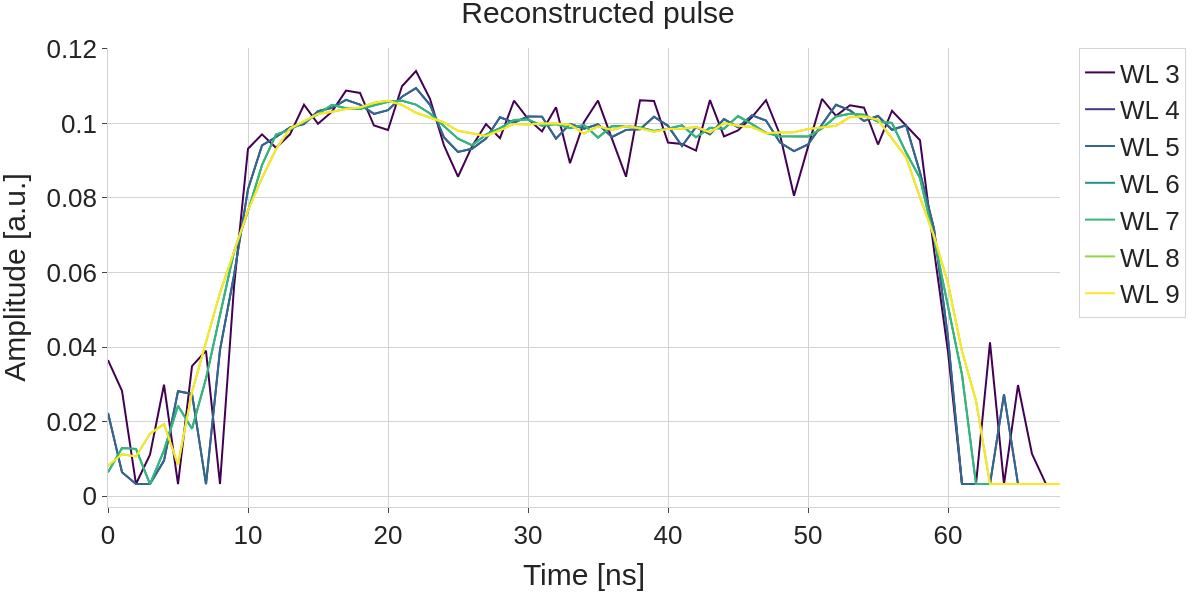
\includegraphics[width=\textwidth]{figures/png/Cryoscope/no_demod/amplitude_windows.png}
        \caption{Flux pulse reconstruction using the cryoscope technique.\\
        The intended pulse has the shape of waveform\_1 and no demodulation was originally applied.}
        \label{fig:amplitude:step_dem}
    \end{subfigure}
    \hfill
    \begin{subfigure}[t]{0.495\textwidth}
        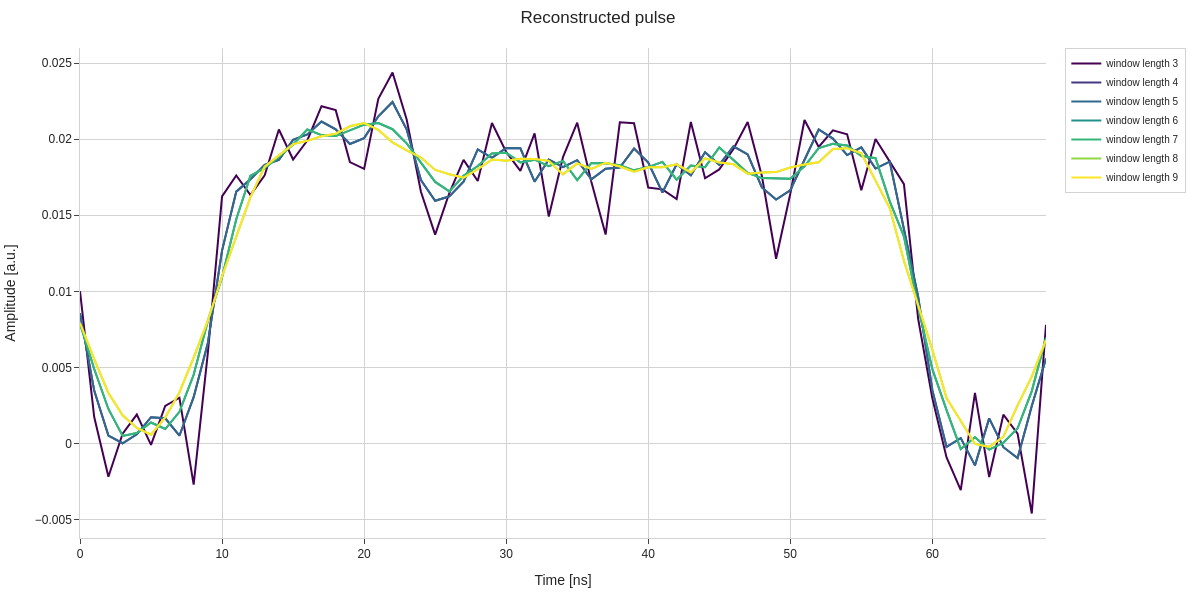
\includegraphics[width=\textwidth]{figures/png/Cryoscope/demodulation/amplitude_windows.png}
        \caption{Flux pulse reconstruction using the cryoscope technique.\\
        The intended pulse has the shape of waveform\_1, demodulation was originally applied.}
        \label{fig:amplitude:step_no_dem}
    \end{subfigure}

    \vspace{0.5cm}

    \begin{subfigure}[t]{0.495\textwidth}
        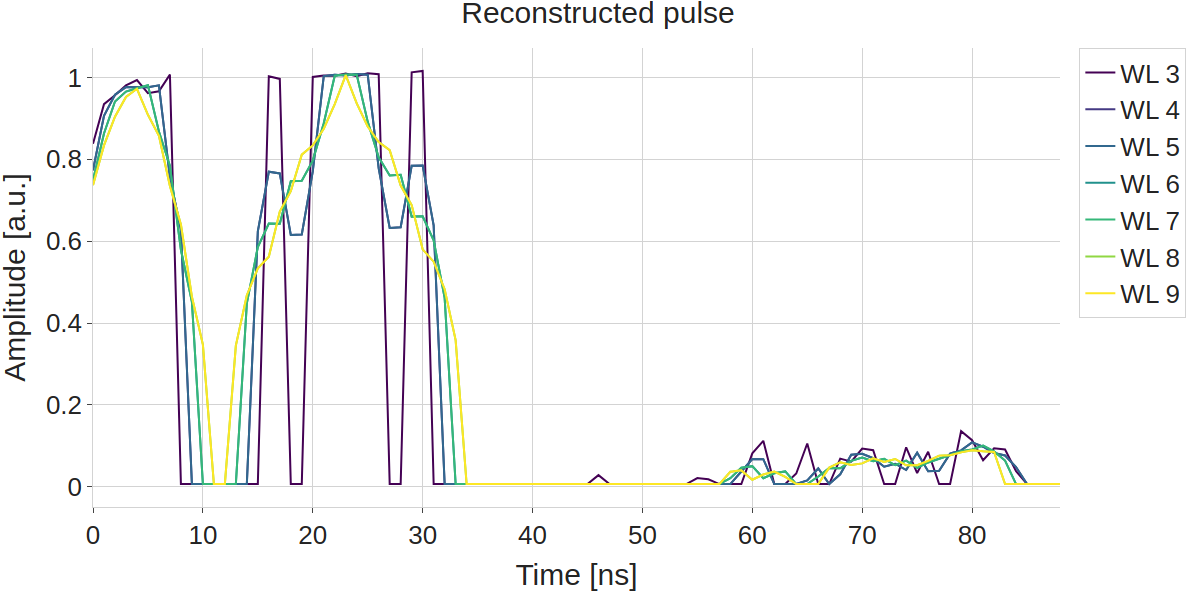
\includegraphics[width=\textwidth]{figures/png/Cryoscope/no_demod/long/amplitude_windows.png}
        \caption{Flux pulse reconstruction using the cryoscope technique.\\
        The intended pulse has the shape of waveform\_2 and no demodulation was originally applied.}
        \label{fig:amplitude:long_no_dem}
    \end{subfigure}
    \hfill
    \begin{subfigure}[t]{0.495\textwidth}
        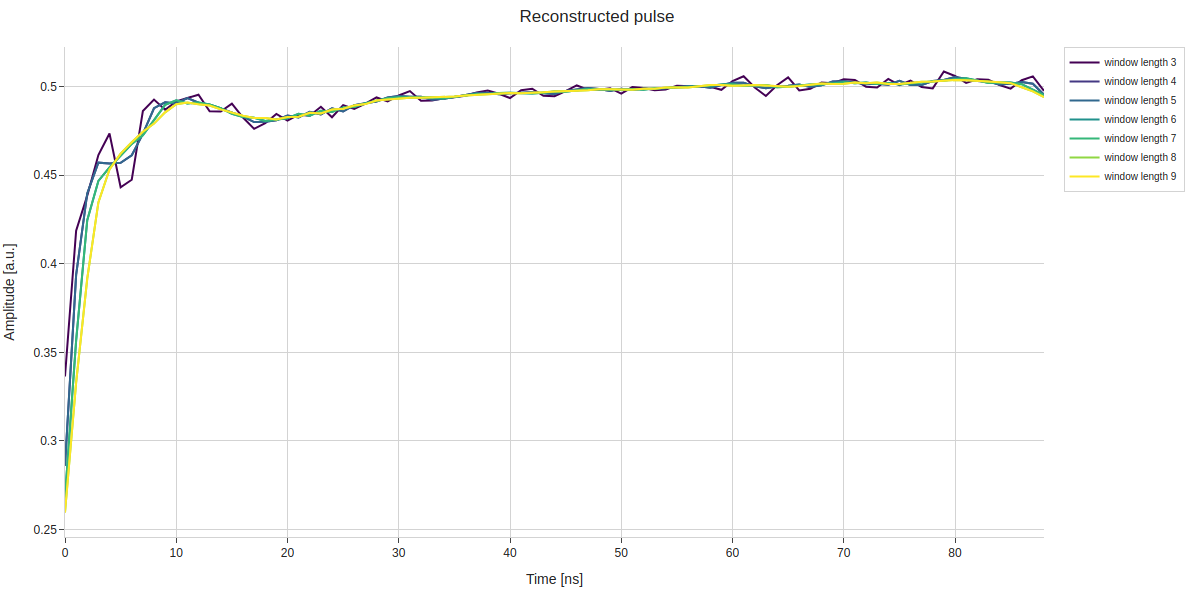
\includegraphics[width=\textwidth]{figures/png/Cryoscope/demodulation/long/amplitude_windows.png}
        \caption{Flux pulse reconstruction using the cryoscope technique.\\
        The intended pulse has the shape of waveform\_2, demodulation was originally applied.}
        \label{fig:amplitude:long_dem}
    \end{subfigure}

    \caption{Examples of reconstruction of the flux amplitude.}
    \label{fig:amplitude}
\end{figure}

Based on the results presented so far regarding the reconstruction of the flux pulse, we chose to adopt a default \tt{window\_length} corresponding to 7 points, similarly to what was done in \cite{rol_time-domain_2020}.

\subsection{Filter determination}
Our goal in implementing the Cryoscope protocol is to determine how to predistort the flux pulse in order to produce the desired detuning on the qubit. 
This predistortion is applied by filtering the waveform generated by the AWG using a combination of FIR and IIR digital filters. 
The goal of these filters is to compensate for the linear-dynamical distortions in the flux control line that would otherwise distort the shape of the pulse as it reaches the qubit.

In practice, the Cryoscope protocol allows us to extract the appropriate feedforward and feedback coefficients that define these filters. 
In the \Qibo setup these coefficients are stored in the platform configuration file (parameters.json) and, once the setup is updated using the \tt{qq update} command, the filters are automatically applied to every flux pulse. 
Since this correction is handled directly by the control hardware, it effectively acts in real-time.

\subsubsection{IIR corrections}

Infinite Impulse Response (IIR) filters are digital filters characterized by the use of both past input samples and feedback from previous output values.
The general form of an IIR filter in discrete time is given by the difference equation:
\begin{equation}
        a_0 y[n] = \sum_{i=0}^{N} b_i x[n - i] - \sum_{i=1}^{M} a_i y[n - i],
\end{equation}
where $x[n]$ is the input signal, $y[n]$ is the output signal, $b_i$ are the feedforward coefficients, $a_i$ are the feedback coefficients, $N$ and $M$ are the orders of the feedforward and feedback components, respectively.

This recursive structure allows IIR filters to approximate systems with exponential or resonant dynamics, which makes them especially suitable for correcting physical distortions like exponential overshoot or undershoot.

Indeed, the first step in our signal correction procedure is to characterize and compensate for the exponential overshoot or undershoot observed in the system's step response. 
These distortions can be interpreted as resulting from the system's impulse response $h(t)$ which when convolved with an ideal step input $V_{in}(t) = V_0\cdot u(t)$, produces the measured output:
\begin{equation}
    s(t) = (h \ast V_{in})(t),
\end{equation}
where $u(t)$ is the Heaviside step function and the system is assumed to be causal ($h(t)=0$ for $t<0$).

In practice, we observe that the system's step response closely follows an exponential form, which we model as:
\begin{equation}
    s(t) = g(1-Ae^{-t/\tau})\cdot u(t),
\end{equation}
where $A$ is the exponential amplitude characterizing the overshoot or undershoot, $\tau$ is the charachteristic time constant and $g$ is a gain factor.

To compensate for this distortion, we construct a digital IIR filter designed to recover an ideal step-like response from the measured signal. 
This is done by modeling the observed step response with an inverted exponential correction function. The corrected signal is then defined as:
\begin{equation}\label{eq:inverse}
s_{\text{corr}}(t) = \frac{s(t)}{g(1 - Ae^{-t/\tau})},
\end{equation}
where $s(t)$ is the measured response. 
The parameters $g, A$, and $\tau$  are estimated by performing a least-squares minimization. 
Specifically, we minimize the squared difference between the corrected signal $s_{\text{corr}}(t)$ and the ideal target signal using \tt{least\_squares} method of the \tt{scipy.optimize} library.

Figures \ref{fig:inverse_short} and \ref{fig:inverse:long} show the results of applying the exponential filters, obtained through the procedure described above, to different flux pulses.

%inverse step
\begin{figure}[h!]
    \centering
    \begin{subfigure}[t]{0.495\textwidth}
        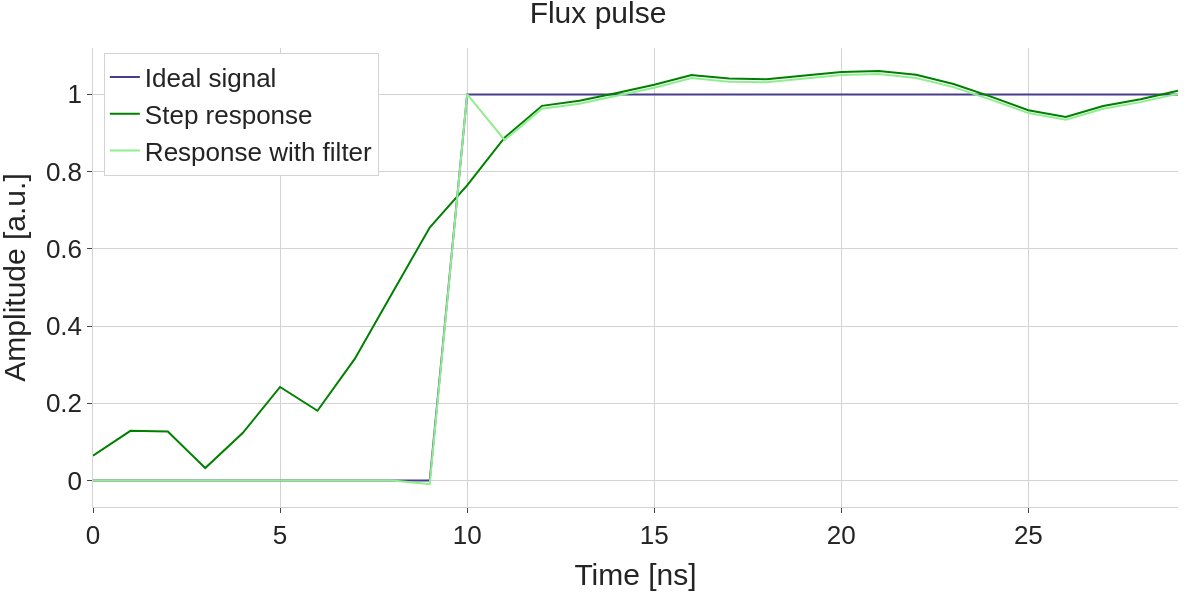
\includegraphics[width=\textwidth]{figures/png/Cryoscope/filters/step_inverse.png}
        \caption{Comparison between the ideal, reconstructed response and corrected flux pulse for a step signal.}
        \label{fig:inverse:step}
    \end{subfigure}
    \hfill
    \begin{subfigure}[t]{0.495\textwidth}
        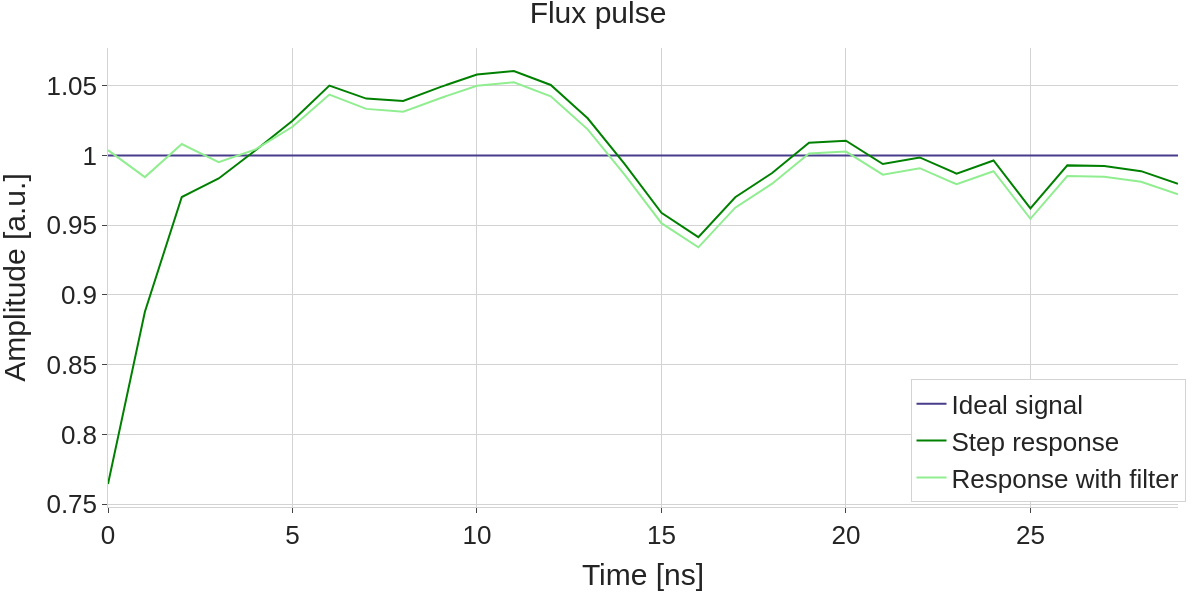
\includegraphics[width=\textwidth]{figures/png/Cryoscope/filters/inverse_no_pad.png}
        \caption{Comparison between the ideal, reconstructed response, and corrected flux pulse for the step signal without the padding.}
        \label{fig:inverse:no_pad}
    \end{subfigure}
    \caption{Comparisons between the ideal flux pulse (blue), the reconstructed flux pulse (dark green), flux pulse after the application of the correction (light green) for different pulse shapes.
    The exponential correction is applied as described in Equation \label{eq:inverse}.}
    \label{fig:inverse_short}
\end{figure}

\begin{figure}[h!]
    \centering
    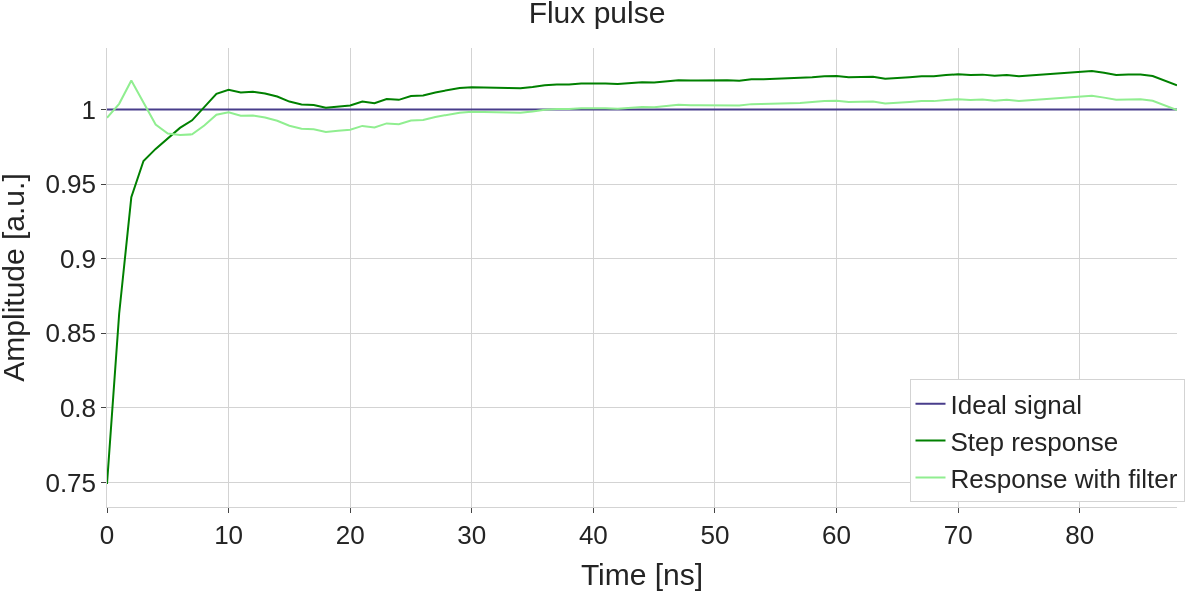
\includegraphics[width=0.5\textwidth]{figures/png/Cryoscope/filters_long/inverse.png}
    \caption{Comparison between the ideal flux pulse (blue), and corrected flux pulse for a rectangular pulse with no padding.}
    \label{fig:inverse:long}
\end{figure}

The first observation from these plots is that the IIR filter effectively compensates for the exponential rise observed in the step response.
%
In particular, for the signals shown in Figure \ref{fig:inverse:step}, the signal-to-noise ratio (SNR)
\footnote{It is worth noting that, in this context, SNR may not be the most appropriate figure of merit; however, it effectively illustrates how the application of a given predistortion improves signal quality.} 
increases from 20 to 547 following the application of the correction.
If we instead consider only the time interval during which the signal is non-zero, as in Figure \ref{fig:inverse:no_pad}, the SNR increases from 305 to 1108.\\
In the acquisition performed using waveform\_2, the signal exhibits significantly reduced distortion compared to the previous case. 
This results in an SNR of 794 for the uncorrected signal, which increases to 19176 following the application of the exponential correction (see Figure \ref{fig:inverse:long}).
%
However, particularly in Figure \ref{fig:inverse:long}, it seems that the filter does not fully eliminate the overshoot. 
A possible explanation for this behavior is that the apparent exponential overshoot may originate from imperfect signal normalization, rather than from an actual residual distortion.
\paragraph{}
After verifying the effectiveness of a single exponential filter, we tried to use a combination of more exponentials to correct flux distortions occurring over time scales ranging from $30$ to $200$ ns, as was suggested in the original work by Rol et al. 
Based on this, we tested the application of multiple exponential corrections of the form given in Equation \ref{eq:inverse}.

\begin{figure}[h!]
    \centering
    \begin{subfigure}[t]{0.495\textwidth}
        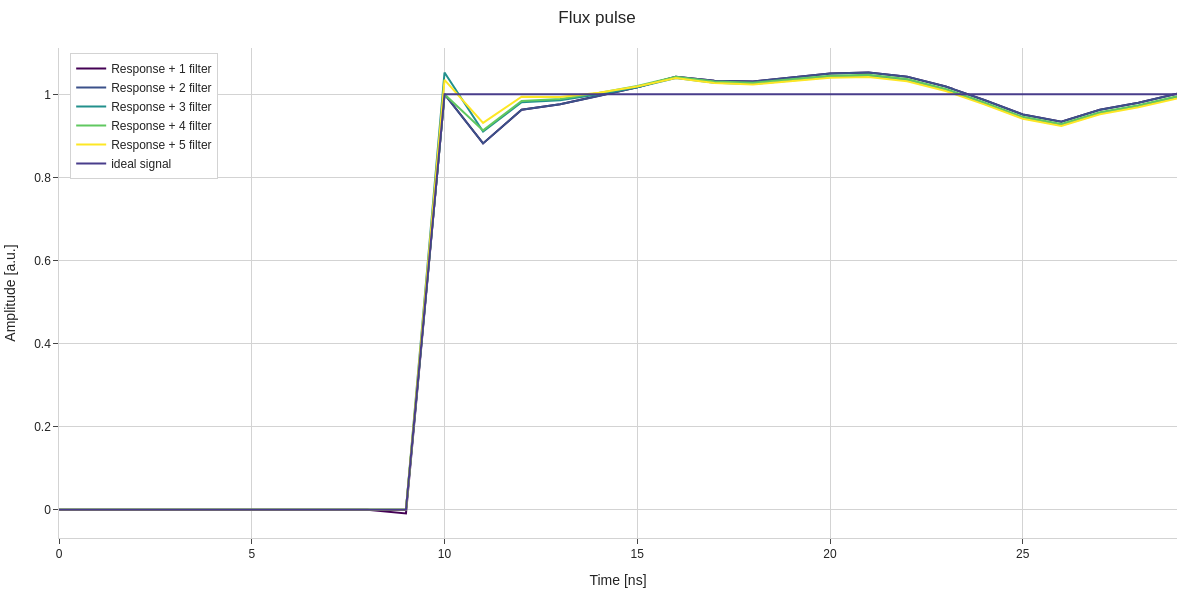
\includegraphics[width=\textwidth]{figures/png/Cryoscope/filters/step_5_inverse.png}
        \caption{Plot of the ideal, reconstructed, and corrected pulse with different numbers of exponential corrections for a step signal.}
        \label{fig:5inverse:step}
    \end{subfigure}
    \hfill
    \begin{subfigure}[t]{0.495\textwidth}
        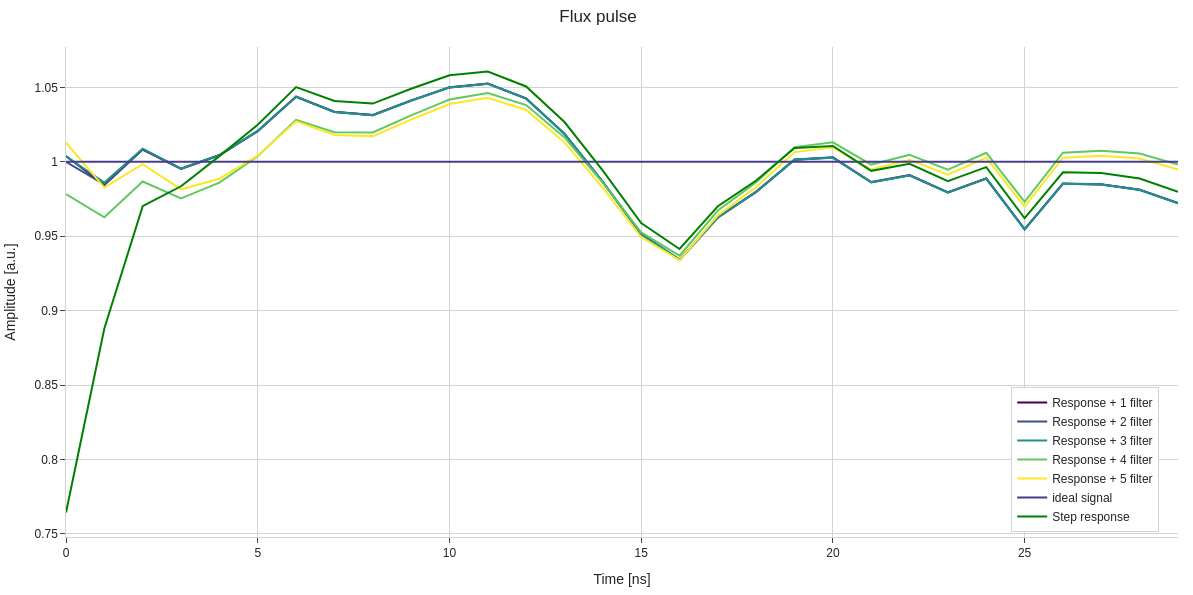
\includegraphics[width=\textwidth]{figures/png/Cryoscope/filters/inverse_5_no_pad.png}
        \caption{Plot of the ideal, reconstructed, and corrected pulse with different numbers of exponential corrections for a step signal without the initial padding.}
        \label{fig:5inverse:no_pad}
    \end{subfigure}
    
    \caption{Comparisons between the ideal flux pulse (blue), the actual flux pulse (dark green), and the flux pulse after the application of a different number of exponential filters for different pulse shapes.
    The correction was applied iteratively, with each step using an exponential function of the form given in Equation \eqref{eq:inverse}.}
    \label{fig:5inverse_short}
\end{figure}

\begin{figure}[h!]
    \centering
    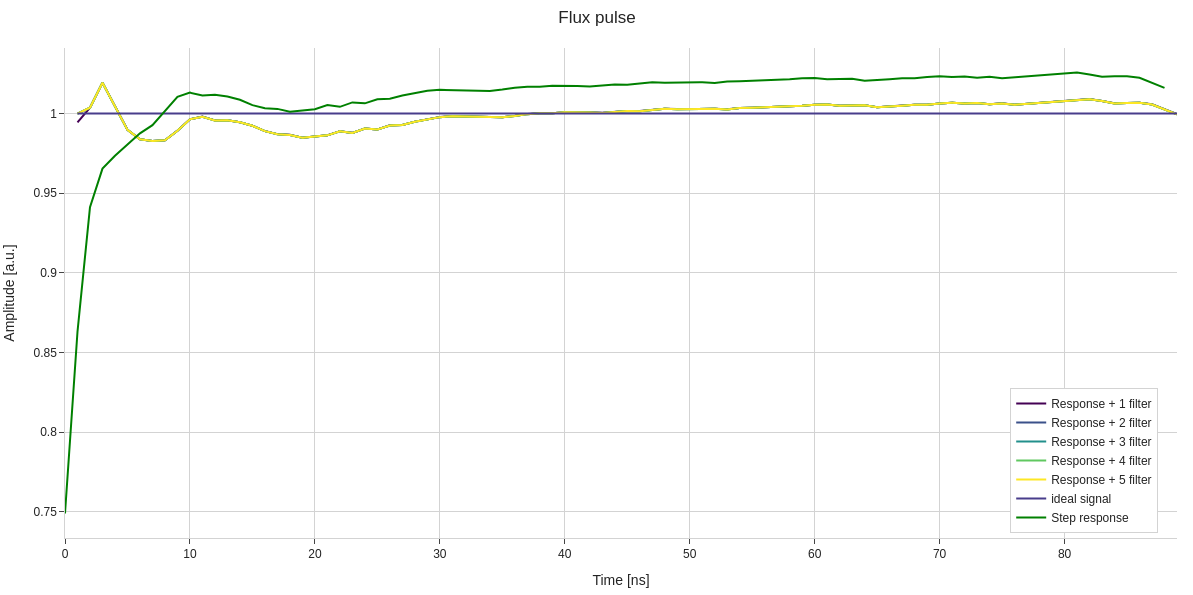
\includegraphics[width=0.5\textwidth]{figures/png/Cryoscope/filters_long/5_inverse.png}
    \caption{Plot of the ideal flux pulse (blue), reconstructed response (dark green), and corrected pulse with different numbers of exponential corrections for a rectangular pulse with no padding.}
    \label{fig:5inverse:long}
\end{figure} 

As shown in Figure \ref{fig:5inverse_short}, the application of successive exponential corrections yields a modest improvement in the reconstructed signal, particularly for the acquisition performed with waveform\_1.
In this case, the SNR obtained at each iteration for the signal shown in Figure \ref{fig:5inverse:no_pad} is, respectively, 1108, 1108, 1109, 1506, and 1676.
In contrast, for the second acquisition, the application of additional exponential filters does not produce a significant enhancement.
After the first correction, the SNR increases from 794 to 19176, as previously noted, but remains essentially unchanged with further iterations.
This difference is likely due to the distinct experimental conditions of the two acquisitions. 
In the first case, the reconstruction of the signal acquired with a \tt{flux\_pulse\_amplitude} of $0.1$ exhibits a more pronounced distortion, which the filters compensate for. 
On the other hand, in the second case, the reconstructed signal already appears much less distorted, reducing the benefit of using more than one exponential correction.

Before presenting the remaining results and continuing with the description of the procedure, it is useful to make the following observation.
The tests on filter performance and the determination of corresponding taps using \tt{waveform\_1} primarily serve as a means to evaluate the effectiveness and limitations of the correction method. 
In this case, the exponential rise corrected by the filters does not reflect a physical property of the system, but rather an artifact introduced by the smoothing behavior of the Savitzky-Golay filter.

To obtain correction taps that address real physical distortions in the flux line, it is necessary to use acquisitions based on \tt{waveform\_2}, which has therefore been selected as the default waveform for the cryoscope protocol. 
This choice ensures a more accurate reconstruction of the system response by avoiding non-physical effects due to pre-pulse padding.

Consequently, in the analyses that follow, we decided to focus exclusively on the non-zero portion of the flux signal. 
Even for the initial acquisitions that include a flat pre-pulse region, this segment has been excluded to ensure that the tests performed with the filters are more meaningful.

At this stage, the parameters for the exponential corrections have been determined. However, to apply these corrections in real-time, they must be discretized and implemented as digital filters within the qubit control electronics. 
Accordingly, the fitted parameters are used to calculate the coefficients of a first-order IIR filter as follows:
\begin{align}
    a_0 &= 1, \\
    a_1 &= -(1 - \alpha), \\
    b_0 &= 1 - k + k \alpha, \\
    b_1 &= -(1 - k)(1 - \alpha),
\end{align}
where 
\begin{equation}
\alpha = 1 - \exp\left(-\frac{1}{f_s \cdot \tau (1 + A)}\right),
\end{equation}
and
\begin{equation}
    k =
    \begin{cases}
    \frac{A}{(1 + A)(1 - \alpha)}, & \text{if } A < 0, \\
    \frac{A}{1 + A - \alpha}, & \text{if } A \geq 0,
    \end{cases}
\end{equation}
with $f_S$ being the sampling frequency of the digital hardware.
Since this is an approximation of the exponential response, we expect the quality of the correction to be somewhat reduced compared to what is achieved by applying the continuous exponential filter.

To predict the effect of applying the real-time predistortion filters, we use the \tt{lfilter} function from the \tt{SciPy} library. 
The function takes three vectors as input: \tt{lfilter(a,b,sig)} and applies the filter defined by the coefficient vectors \tt{b} and \tt{a} to the signal represented by the vector \tt{sig}. 
The results of applying these IIR filters as discrete digital filters are shown in Figure \ref{fig:IIR}.

\begin{figure}[h!]
    \centering
    \begin{subfigure}[t]{0.495\textwidth}
        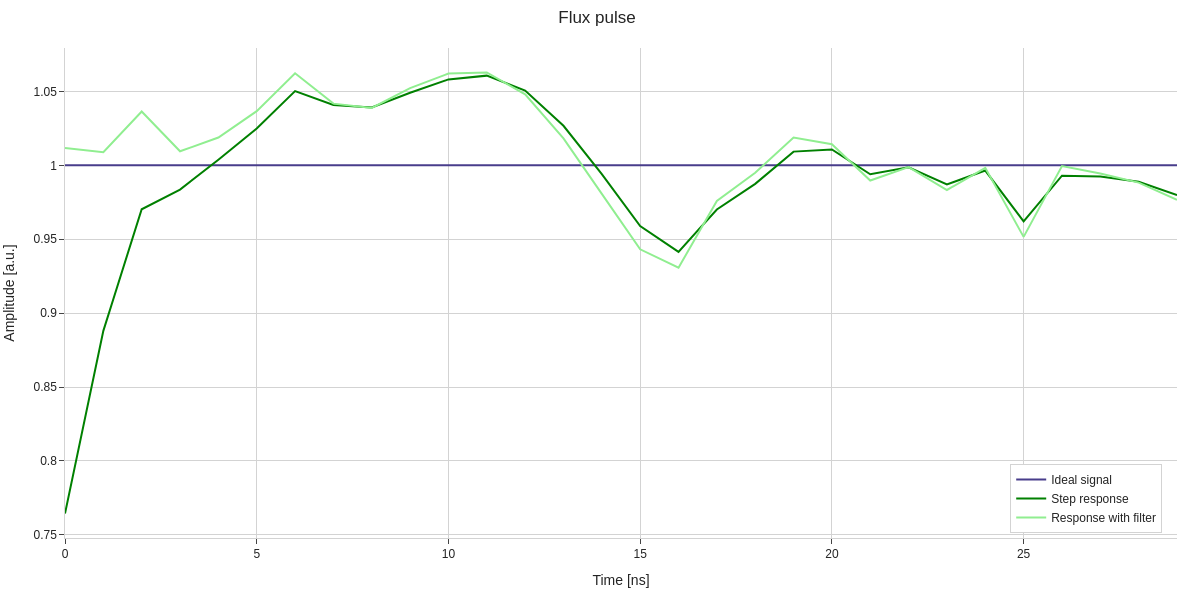
\includegraphics[width=\textwidth]{figures/png/Cryoscope/filters/IIR_nopad.png}
        \caption{Plot of the ideal, reconstructed, and corrected pulse for a step signal without the initial padding and a $0.1$ flux pulse amplitude.}
        \label{fig:IIR:nopad}
    \end{subfigure}
    \hfill
    \begin{subfigure}[t]{0.495\textwidth}
        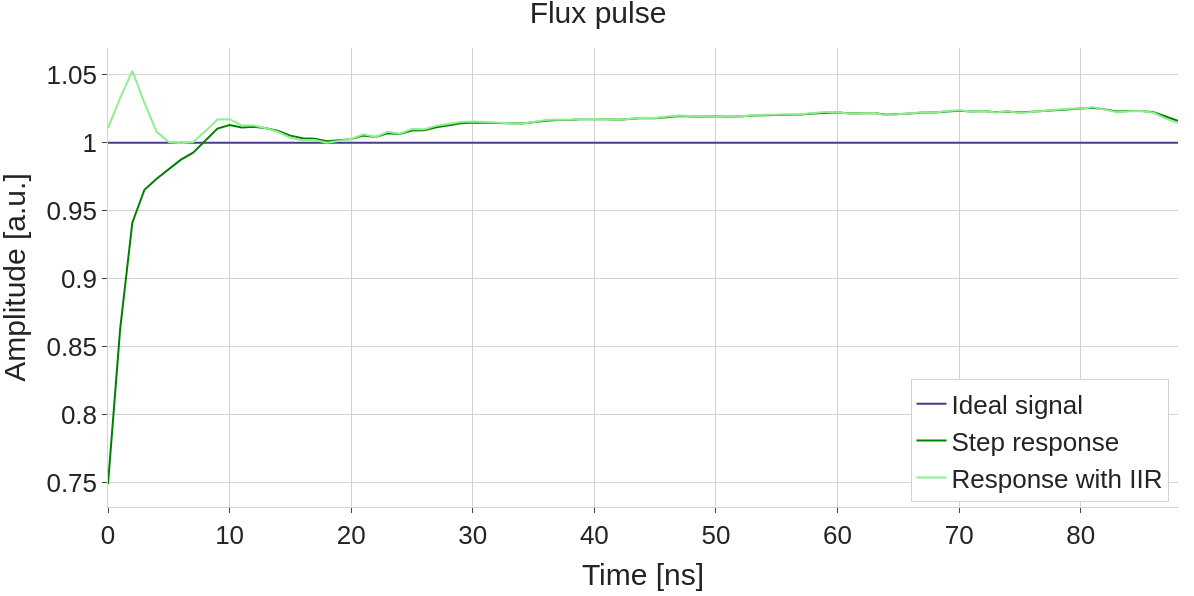
\includegraphics[width=\textwidth]{figures/png/Cryoscope/filters_long/IIR.png}
        \caption{Plot of the ideal, reconstructed, and corrected pulse for a rectangular pulse with no padding and a $0.5$ flux pulse amplitude.}
        \label{fig:IIR:long}
    \end{subfigure}
    \caption{Comparisons between the ideal flux pulse (blue), the actual flux pulse (dark green), flux pulse after the application of the discrete IIR corrections (light green) for different flux pulses.}
    \label{fig:IIR}
\end{figure}

As expected, the quality of the correction obtained using the IIR digital filter is lower compared to that achieved by applying the exponential correction via inversion (as in Equation \ref{eq:inverse}). 
This is evidenced by the resulting SNR: in the first case, the application of the IIR filter yields an SNR of 833, compared to 1108 obtained with the previous method.
In the second case, the SNR increases from 1976 to 2867 following the IIR correction. 
Although this represents a noticeable reduction in performance relative to the inversion-based approach, the resulting SNR remains remarkably high.

\subsubsection{FIR corrections}
Once the feedback and feedforward taps for the IIR filters have been determined, it is necessary to implement a finite impulse response (FIR) filter to correct for residual distortions on shorter timescales, less than 30 ns, which are not fully addressed by the IIR.
A Finite Impulse Response (FIR) filter produces its output as a weighted sum of the current and a finite number of past input samples. It is mathematically defined by
\begin{equation}
        y[n] = \sum_{i=0}^{N} b_i x[n - i],
\end{equation}
where $x[n]$ is the input signal and $y[n]$ is the output signal of the filter.

The filter coefficients are obtained by minimizing the average relative deviation between the filtered output (the result of applying the FIR filter to the signal already corrected by the IIR filter) and the ideal step response. 
This optimization is carried out using the \tt{CMA-ES} algorithm (for further details on the \tt{CMA-ES} algorithm, see Section \ref{sec:CMA}).

In the implementation for \Qibocal, the number of FIR filter taps can be selected by the user via the \tt{fir} parameter. 
For our initial tests, we chose to use 20 taps.\\
Given that the OPX1000 controller for the qw11q operates at a sampling rate of $1$ GSa/s, this corresponds to one tap per nanosecond. 
Accordingly, in these initial tests, we optimized 20 parameters to determine the 20 filter taps.

The results of applying the FIR filters are shown in Figure \ref{fig:FIR}. 
Specifically, Figure \ref{fig:FIR:nopad} displays the results of applying the FIR filter to the flux pulse generated using waveform\_1, while Figure \ref{fig:FIR:long} shows the corresponding results for the flux pulse generated with waveform\_2. 
Both sets of filtered signals were obtained using the \tt{lfilter} function from the \tt{SciPy} library.

\begin{figure}[h!]
    \centering
    \begin{subfigure}[t]{0.495\textwidth}
        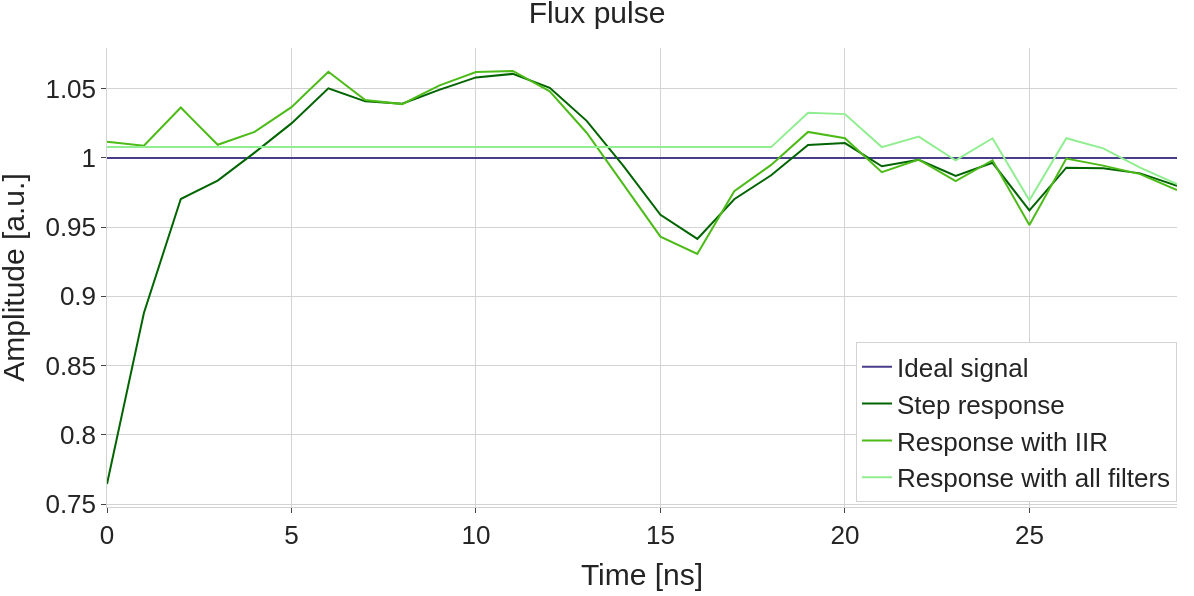
\includegraphics[width=\textwidth]{figures/png/Cryoscope/filters/all_filters_no_pad.png}
        \caption{Plot of the ideal, reconstructed, and corrected pulse for a step signal without the initial padding and a $0.1$ flux pulse amplitude.}
        \label{fig:FIR:nopad}
    \end{subfigure}
    \hfill
    \begin{subfigure}[t]{0.495\textwidth}
        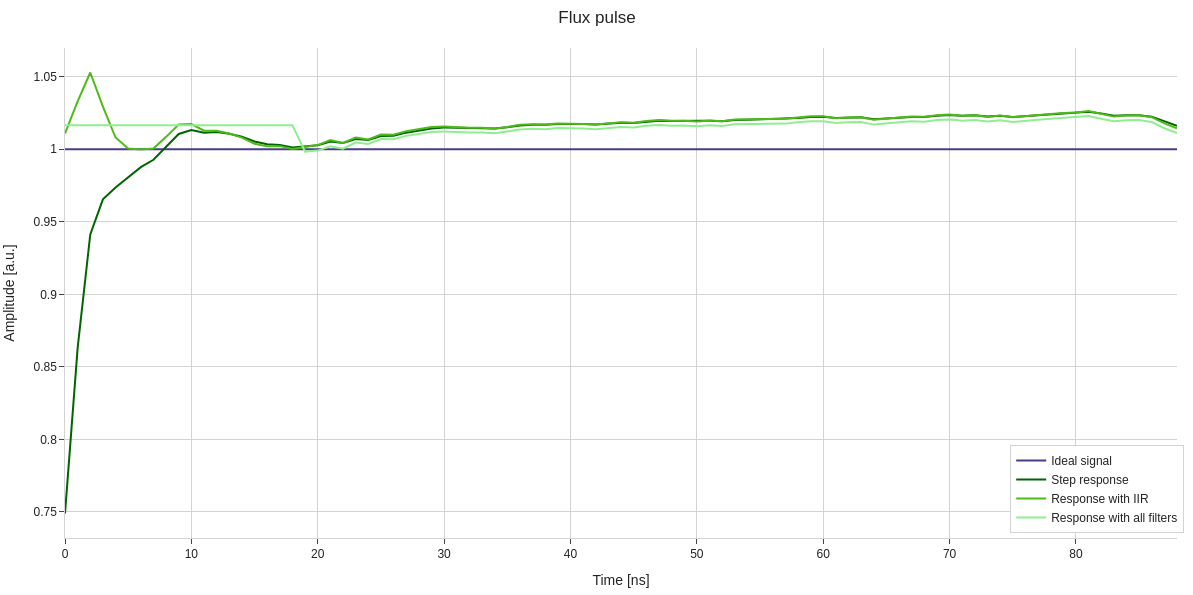
\includegraphics[width=\textwidth]{figures/png/Cryoscope/filters_long/IIR_FIR.png}
        \caption{Plot of the ideal, reconstructed, and corrected pulse for a rectangular pulse with no padding and a $0.5$ flux pulse amplitude.}
        \label{fig:FIR:long}
    \end{subfigure}
    \caption{Comparisons between the ideal flux pulse (blue), the actual flux pulse (dark green), the flux pulse after the application of the discrete IIR corrections (green), and both IIR and FIR corrections (light green) for different flux pulses.}
    \label{fig:FIR}
\end{figure}

The first observation, consistent with the results shown in Figures \ref{fig:inverse_short}, \ref{fig:inverse:long}, and \ref{fig:IIR}, is that there may be an issue with signal normalization that we are not addressing yet. 
This is evident because, in theory, the FIR filter coefficients are optimized to bring the filtered flux signal as close as possible to unity. 
However, the results show that even where the FIR filters should adjust the signal to exactly one, the value remains slightly above unity.

A second important consideration concerns the correction strategy. 
When the number of parameters optimized equals the number of FIR filter coefficients, and this coincides with the number of signal samples, there is effectively a one-to-one mapping between optimized parameters, filter coefficients, and signal points. 
This means that the optimization is essentially adjusting the signal point-by-point to match the desired target values. 
Although this procedure yields a close fit to the reference signal, its practical utility is limited, particularly because the signal used for optimization is pre-recorded rather than acquired in real-time. 
As a result, future signals may exhibit different features, reducing the generalizability of the resulting filter.

To improve robustness, it is preferable to reduce the number of free parameters in the optimization.
A finer-grained optimization, where individual parameters are assigned to each filter coefficient and time sample—can be restricted to the initial portion of the response (approximately the first 5 ns) where the distortions due to the IIR filters are most pronounced.
Beyond this interval, a coarser parameterization can be adopted by grouping adjacent FIR coefficients under a single optimization parameter.
This strategy reduces the dimensionality of the problem while promoting a more general filter profile, better suited for correcting distortions in signals that differ from the original reference.

As a practical example, we repeated the FIR coefficient optimization using 17 parameters with the \tt{CMA-ES} algorithm. 
The first 4 parameters correspond directly to the first 4 FIR coefficients, while the remaining 13 parameters each control two coefficients, effectively determining 26 coefficients. 
Given the 1 GSa/s sampling rate, this approach optimizes the correction over a time window of approximately 30 ns. 
The results of this improved optimization are shown in Figure \ref{fig:nice}.

\begin{figure}[h!]
    \centering
    \begin{subfigure}[t]{0.495\textwidth}
        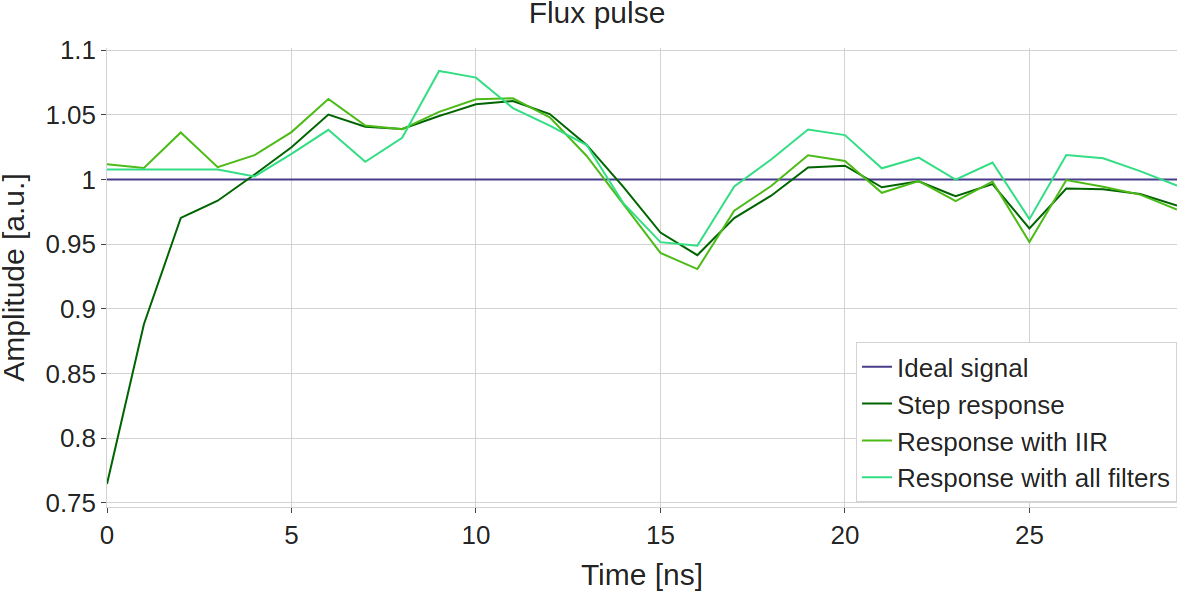
\includegraphics[width=\textwidth]{figures/png/Cryoscope/step_nice.png}
        \caption{Plot of the ideal, reconstructed, and corrected pulse for a step signal without the initial padding and a $0.1$ flux pulse amplitude.}
        \label{fig:nice:nopad}
    \end{subfigure}
    \hfill
    \begin{subfigure}[t]{0.495\textwidth}
        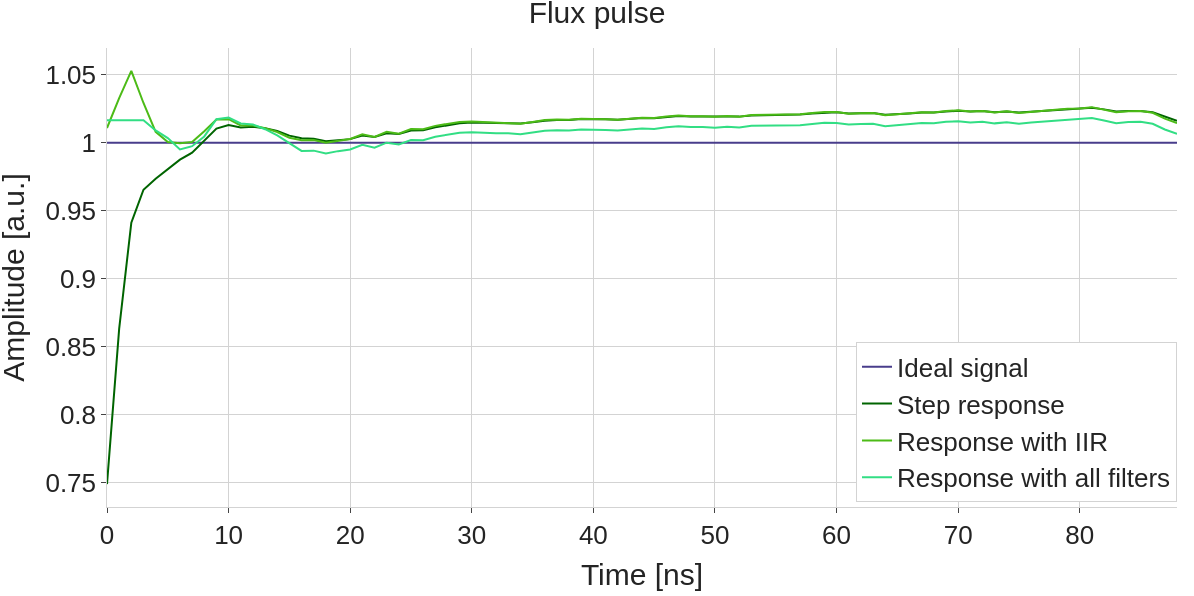
\includegraphics[width=\textwidth]{figures/png/Cryoscope/long_nice.png}
        \caption{Plot of the ideal, reconstructed, and corrected pulse for a rectangular pulse with no padding and a $0.5$ flux pulse amplitude.}
        \label{fig:nice:long}
    \end{subfigure}
    \caption{Comparisons between the ideal flux pulse (blue), the actual flux pulse (dark green), the flux pulse after the application of the discrete IIR corrections (green), and both IIR and FIR corrections (light green) for different flux pulses.}
    \label{fig:nice}
\end{figure}

As expected, the application of FIR filters leads to a clear improvement in signal quality. 
For the traces shown in Figure \ref{fig:nice:nopad}, the SNR increases from 833 to 951 in the first case, and from 2867 to 7338 in the second.

\subsubsection{Output filters in QM}

Each analog output port of the OPX system used in this work is equipped with a digital filter that is applied to the signal in the digital domain before conversion to analog. 
Using the output filter, we can attend to the unwanted effects of the different electrical components of the setup without altering our waveforms.

Using \Qibolab the filters are provided to the OPX via the \tt{parameters.json} file, which contains the coefficients for the feedforward and feedback components according to the equation
\begin{equation}\label{eq:OPX_filter}
    y[n] = \sum_{m=1}^{M} a_m y[n - m] + \sum_{k=0}^{K} b_k x[n - k],
\end{equation}
where $y[n]$ is the output signal, $x[n]$ is the input waveform, $a_m$ are the feedback coefficients, and $b_k$ are the feedforward coefficients.

In our case, we have a set of feedback coefficients determined through IIR correction and two sets of feedforward coefficients: the first obtained from the IIR-based correction, and the second from FIR-based correction on short timescales. 
To uniquely determine the coefficients to be passed to the electronics, it is necessary to derive a single set of feedforward coefficients and a single set of feedback coefficients by combining the two sets of feedforward filters through convolution.

Indeed, we can consider the input signal $x$ to which we apply a first IIR filter, thus obtaining an output signal $y$ such that 
\begin{equation}\label{eq:y_signal}
    y[n] = \sum_{m=1}^{M} a[m]y[n-m] + \sum_{k=0}^{N} b[k] x[n-k].
\end{equation}

If we apply a second IIR filter to the $y$ signal we obtain a $z$ signal as output, that can be written as 
\begin{equation}\label{eq:z_signal}
    z[n] = \sum_{m=1}^{M} a'[m]z[n-m] + \sum_{k=0}^{N} b'[k] y[n-k].
\end{equation}

Now we consider Equation \ref{eq:y_signal} and rewrite it as
\begin{equation}\label{eq:y_signal1}
    y[n] - \sum_{m=1}^{M} a[m]y[n-m] = \sum_{k=0}^{N} b[k] x[n-k],
\end{equation} 
then by applying a Z-transform, we obtain
\begin{equation}\label{eq:y_signal_transform}
    Y(z)\left(1 - \sum_{m=1}^{M} a[m] z^{-m} \right) = X(z) \left( \sum_{k=0}^{N} b[k] z^{-k} \right)
\end{equation}
so that 
\begin{align}
    H_1(z) &= \frac{Y(z)}{X(z)} = \frac{\sum_{k=0}^{N} b[k] z^{-k}}{1 - \sum_{m=1}^{M} a[m] z^{-m}} = \frac{B(z)}{A(z)} \\
    & \rightarrow Y(z) = H_1(z)X(z) = \frac{B(z)}{A(z)}X(z) \label{eq:transfer1}
\end{align}

We can do the same also for Equation \ref{eq:z_signal} and rewrite it as 
\begin{equation}\label{eq:z_signal1}
    z[n] = \sum_{m=1}^{M} a'[m]z[n-m] + \sum_{k=0}^{N} b'[k] y[n-k],
\end{equation}
which, by applying the Z-transform becomes
\begin{equation}\label{eq:z_signal_transform}
    Z(z)\left(1 - \sum_{m=1}^{M} a'[m] z^{-m} \right) = Y(z) \left( \sum_{k=0}^{N} b'[k] z^{-k} \right).
\end{equation}
Again we can write the the transfer function
\begin{align}
    &H_2(z) = \frac{Z(z)}{Y(z)} = \frac{\sum_{k=0}^{N} b'[k] z^{-k}}{1 - \sum_{m=1}^{M} a'[m] z^{-m}} = \frac{B'(z)}{A'(z)} \\
    \rightarrow Z(z) &= H_2(z)Y(z) = \frac{B'(z)}{A'(z)}Y(z) = \frac{B'(z)}{A'(z)} \frac{B(z)}{A(z)} X(z)\\ \label{eq:transfer2}
    &= \left( \frac{\sum_{k=0}^{N} b'[k] z^{-k}}{1 - \sum_{m=1}^{M'} a'[m] z^{-m}} \right) \left( \frac{\sum_{k=0}^{N} b[k] z^{-k}}{1 - \sum_{m=1}^{M} a[m] z^{-m}} \right) X(z)
\end{align}
From the transfer function we can obtain the expression for $Z(z)$ in terms of $X(z)$ 
\begin{align}
    & \rightarrow Z(z) \left(1 - \sum_{m=1}^{M} a'[m] z^{-m} \right) \left(1 - \sum_{m=1}^{M} a[m] z^{-m} \right) = \left( \sum_{k=0}^{N} b'[k] z^{-k} \right) \left( \sum_{k=0}^{N} b[k] z^{-k} \right) X(z) \\
    & \rightarrow Z(z) \left( \sum_{m=0}^{M} a'[m] z^{-m} \right) \left( \sum_{m=0}^{M} a[m] z^{-m} \right) = \left( \sum_{k=0}^{N} b'[k] z^{-k} \right) \left( \sum_{k=0}^{N} b[k] z^{-k} \right) X(z) \label{eq:Zz}
\end{align}
where in the last step, the term 1 has been absorbed into the summation as the coefficient $a_0$. By expanding the products, we obtain:
\begin{align}
    & \left( \sum_{m=0}^{M} a'[m] \right) \left( \sum_{m=0}^{M} a[m] \right) = \sum_{m=0}^{2M}\sum_{i=0}^{m} a'[i] a[m - i] = c[k], \quad\quad \text{with}\quad m = 0, \dots, 2M, \label{eq:ck} \\
    & \left( \sum_{k=0}^{N} b'[k] \right) \left( \sum_{k=0}^{N} b[k] \right) = \sum_{k=0}^{2N} \sum_{i=0}^{k} b[i] b[k-i] = d[k], \quad\quad \text{with}\quad k = 0, \dots, 2N. \label{eq:dk}
\end{align}
%so that
%\begin{align}
%    & \left( \sum_{m=0}^{M} a'[m] z^{-m} \right) \left( \sum_{m=0}^{M} a[m] z^{-m} \right) = \sum_{m=0}^{2M} c[m]z^{-m} = \sum_{m=0}^{2M}\sum_{i=0}^{m} a'[i]a[m - i]z^{-m}\\
%    & \left( \sum_{k=0}^{N} b'[k] z^{-k} \right) \left( \sum_{k=0}^{N} b[k] z^{-k} \right) = \sum_{k=0}^{2N} d[k]z^{-k} = \sum_{k=0}^{2N}\sum_{i=0}^{k} b'[k]b[k-i]z^{-k}.\\
%\end{align}

It is then possible to re-write equation \ref{eq:Zz} using the new expression for the filters
\begin{align}
    & Z(z)\left( \sum_{m=0}^{2M} c[m]z^{-m} \right) = \left( \sum_{k}^{2N} d[k]z^{-k} \right)X(z)\\
    & \rightarrow Z(z)\left(1 - \sum_{m=1}^{2M} c[m]z^{-m} \right) = \left( \sum_{k}^{2N} d[k]z^{-k} \right)X(z) \label{eq:z_final}
\end{align} 

then we apply the inverse-Z-transform and obtain
\begin{align}
    & z[n] - \sum_{m=1}^{2M} c[m]z[n-m] = \sum_{k=0}^{2N} d[k] x[n-k]\\
    & z[n] = \sum_{m=1}^{2M} c[m]z[n-m] + \sum_{k=0}^{2N} d[k] x[n-k]
\end{align}
where the feedforward (feedback) taps of the final filters, are given by the convolution of the feedforward (feedback) taps of the two filters as shown in Equation \ref{eq:ck} and Equation \ref{eq:dk}.

\subsection{Results}

\begin{figure}[h!]
    \centering
    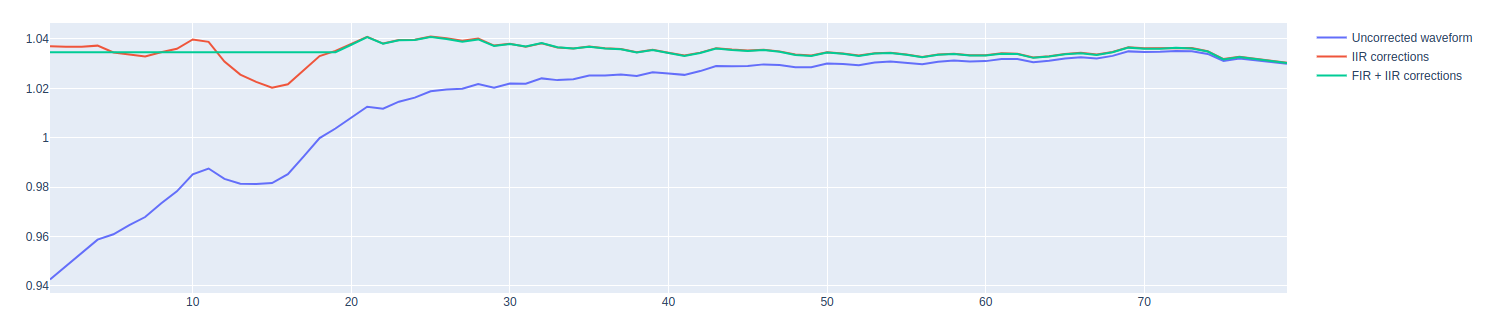
\includegraphics[width=\textwidth]{figures/png/Cryoscope/B3.png}
    \caption{Output of the cryoscope routine on qubit \tt{B3}.}
    \label{fig:cryoscope:B3}
\end{figure} 

Figure \ref{fig:cryoscope:B3} shows the result of the cryoscope routine executed on qubit \tt{B3}. 
As previously discussed, the application of a single IIR filter is sufficient to correct the exponential rise in the step response. 
However, on longer timescales, residual oscillations remain that are not addressed by either the IIR or FIR filters.

While we could attempt to mitigate these effects by combining multiple IIR and FIR filters, the remaining signal distortions appear to be oscillatory in nature and are likely due to ringing phenomena, transient oscillations that typically arise from impedance mismatches, or resonant components in the control line.
These ringing effects are particularly evident in the acquisitions shown in Figure \ref{fig:cryoscope:B2} and \ref{fig:cryoscope:B4}, and persist even after the application of corrective filtering, as confirmed by the reconstructed flux pulses displayed in Figures \ref{fig:flux:B2} and \ref{fig:flux:B4}.
These plots show the reconstructed flux pulse when the digital filters determined with the cryoscope routine are applied, we can see that the oscillations decay in amplitude over time and appear to vanish after approximately 75ns. 

\begin{figure}[h!]
    \centering
    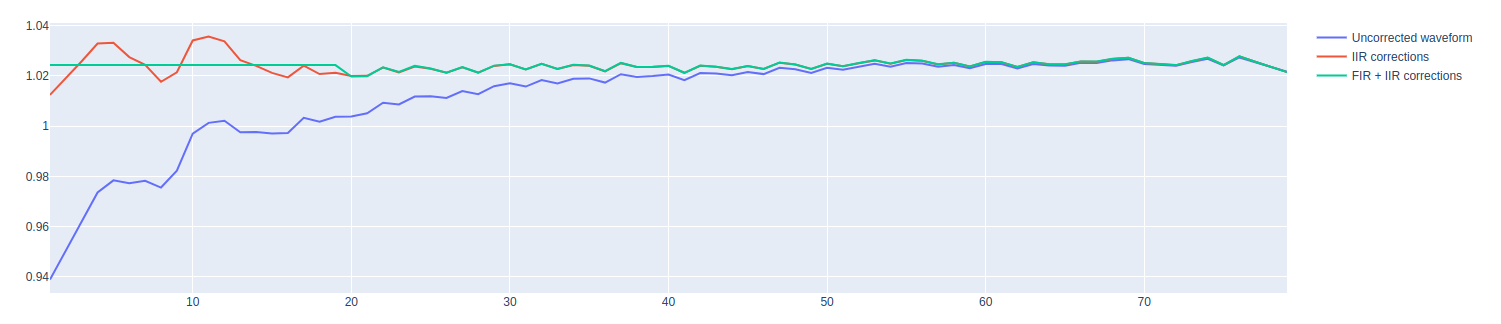
\includegraphics[width=\textwidth]{figures/png/Cryoscope/B2_ringing.png}
    \caption{Output of the cryoscope routine on qubit \tt{B2}.}
    \label{fig:cryoscope:B2}
\end{figure}

\begin{figure}[h!]
    \centering
    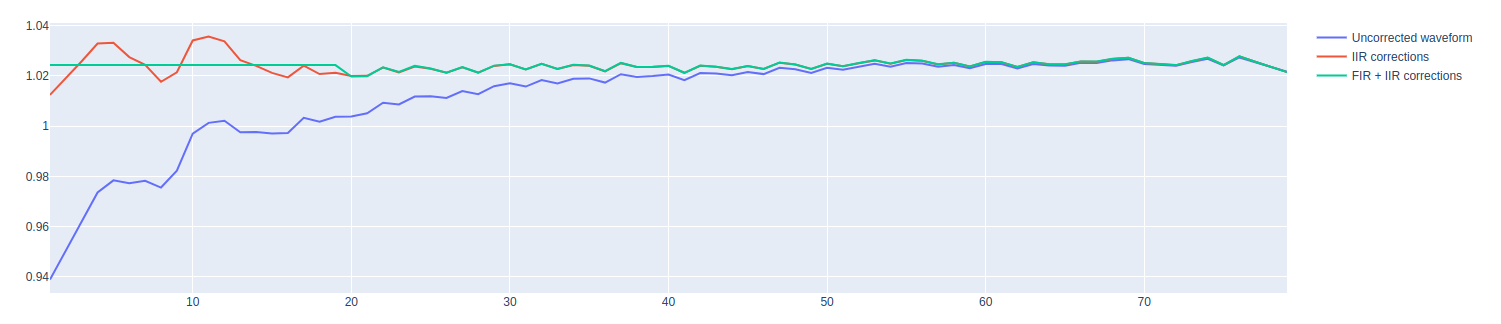
\includegraphics[width=\textwidth]{figures/png/Cryoscope/B2_ringing.png}
    \caption{Output of the cryoscope routine on qubit \tt{B4}.}
    \label{fig:cryoscope:B4}
\end{figure} 

\begin{figure}[h!]
    \centering
    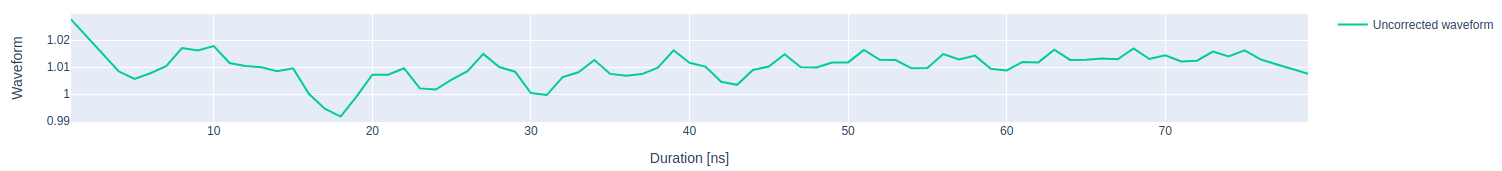
\includegraphics[width=\textwidth]{figures/png/Cryoscope/flux_B2.png}
    \caption{Flux pulse reconstruction for qubit \tt{B2}.}
    \label{fig:flux:B2}
\end{figure}

\begin{figure}[h!]
    \centering
    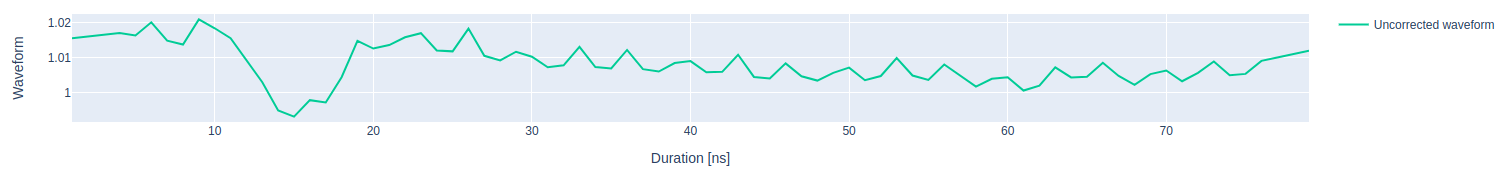
\includegraphics[width=\textwidth]{figures/png/Cryoscope/flux_B4.png}
    \caption{Flux pulse reconstruction for qubit \tt{B4}.}
    \label{fig:flux:B4}
\end{figure} 

\paragraph{}
Experiments in which flux signal distortions are particularly evident are those where a well-defined chevron pattern is expected. Deviations from the ideal chevron structure often indicate the presence of flux distortions in the control signal \cite{Langford2017}.

An example of such an experiment is the routine referred to as chevron in \Qibocal. The name derives from the characteristic chevron-shaped interference pattern that serves as the expected output of the protocol.
This calibration routine is used to characterize and tune native two-qubit gates, such as the CNOT or iSWAP, which are typically implemented using sequences of flux pulses, possibly applied to multiple qubits, combined with virtual $Z$-rotations.
Both CNOT and iSWAP are entangling gates: the CNOT gate flips the state of the target qubit conditional on the control qubit being in the $\ket{1}$ state, while the iSWAP gate exchanges the quantum states $\ket{10} \leftrightarrow \ket{01}$, introducing a phase factor of $i$.

For example, we can consider the pulse sequence used to calibrate the iSWAP gate between a pair of qubits consists of a $\pi$ pulse followed by a flux pulse of varying amplitude and duration, applied to the qubit with the highest frequency in the pair. 
The initial $\pi$ pulse brings the qubit into the state $\ket{1}$, while the flux pulse detunes its frequency near resonance with the second qubit. 

The iSWAP gate exploits the coherent exchange of excitations between two capacitively coupled qubits by tuning them into resonance via a flux pulse. 
When brought into resonance, the computational basis states $\ket{10}$ and $\ket{01}$ become energetically near-degenerate and interact via the coupling, resulting in a level repulsion characteristic of an avoided crossing.
In this regime the population oscillates between the two states with a frequency determined by the coupling strength $g$; the expected population oscillation pattern follows:
\begin{equation}
    p_e(t, \Delta) = \frac{\Delta^2}{\Delta^2 + 4g^2} + \frac{4g^2}{\Delta^2 + 4g^2} \cos^2\left(\frac{\sqrt{\Delta^2 + 4g^2}}{2}t\right)
\end{equation}
where $\Delta = \omega_1 - \omega_2$ is the detuning between the two qubits, and $g$ is the coupling constant. This probability distribution precisely describes what is commonly referred to in the literature as the chevron pattern.

In \texttt{Qibocal}, this routine is used to calibrate native two-qubit gates. For instance, by adjusting the duration $t$ of the flux pulse such that $t = \pi/2g$ the system undergoes a complete excitation exchange, effectively implementing an iSWAP gate up to local phase corrections.  
If, instead, the goal is to calibrate a CZ gate, the pulse sequence remains the same, with the only difference being the inclusion of an initial $\pi$-pulse applied to the lower-frequency qubit. This ensures that both qubits are initially prepared in the $\ket{1}$ state.

The ideal chevron pattern is shown in Figure \ref{fig:expected_chevron}, the figure is meant to give a qualitative idea of how the chevron plot should look like, the scale is different from the real system.

\begin{figure}[h!]
    \centering
    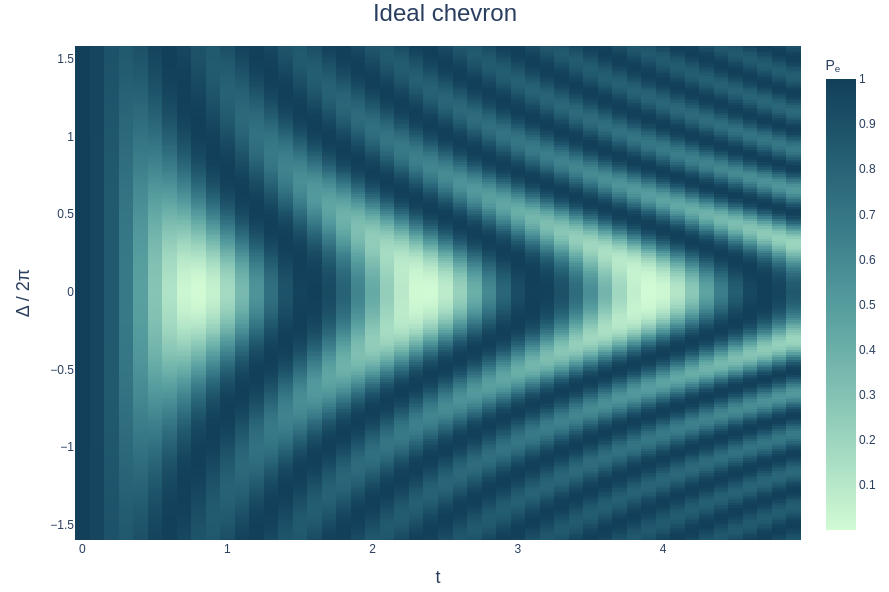
\includegraphics[width=0.5\textwidth]{figures/png/IdealChevron.png}
    \caption{Ideal chevron pattern.}
    \label{fig:expected_chevron}
\end{figure}

\newpage
\newgeometry{a4paper, top=2.5cm, bottom=2.5cm, inner=2cm, outer=2cm, heightrounded}
Figure \ref{fig:B1B3_nofilter} and Figure \ref{fig:B2B4_nofilter} show the actual chevron pattern obtained from the calibration of a CZ gate on our hardware without applying any digital filter.

\begin{figure}[h!]
    \centering
    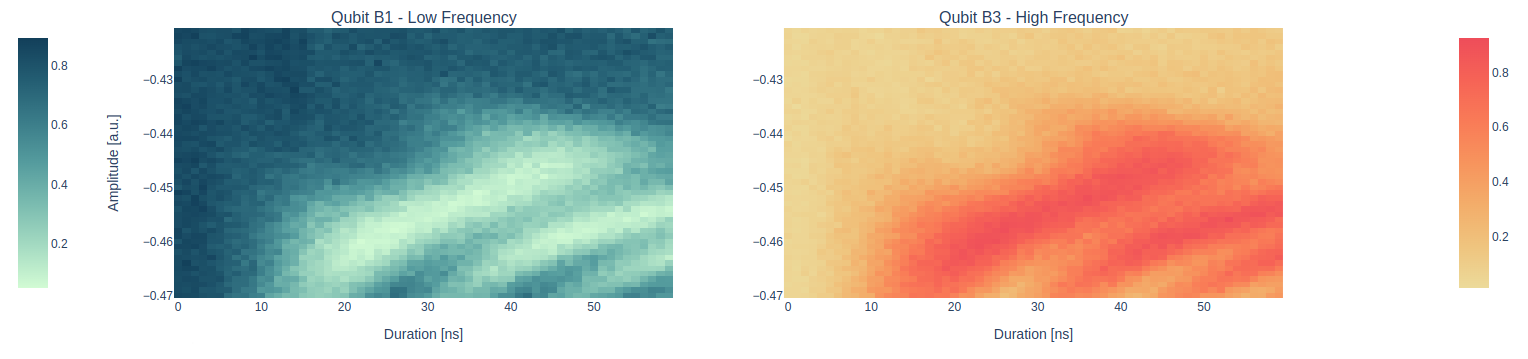
\includegraphics[width=\textwidth]{figures/png/Cryoscope/B1B3_nofilter.png}
    \caption{Chevron pattern obtained from the calibration of a CZ gate on qubits \tt{B1} and \tt{B3}.\\ No filters applied.}
    \label{fig:B1B3_nofilter}
\end{figure}

\begin{figure}[h!]
    \centering
    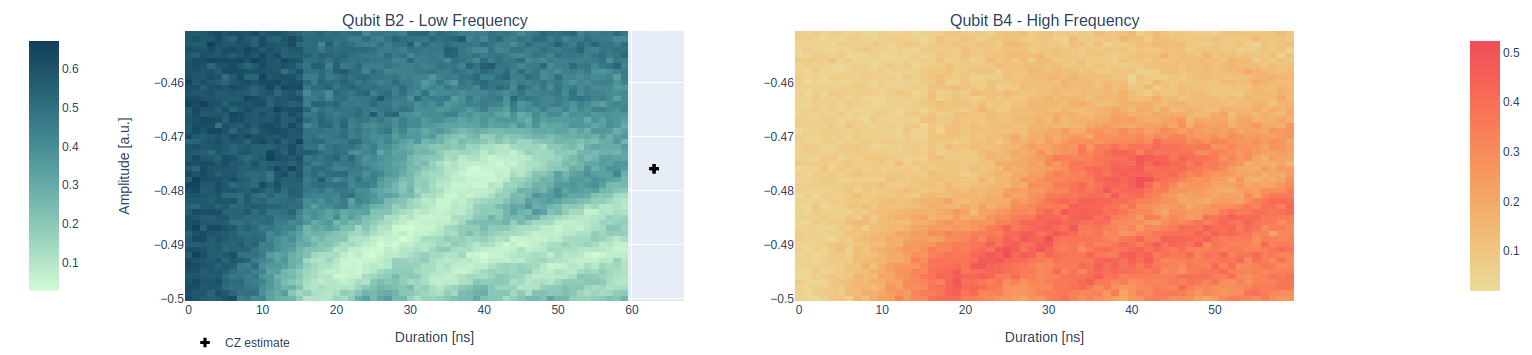
\includegraphics[width=\textwidth]{figures/png/Cryoscope/B2B4_nofilter.png}
    \caption{Chevron pattern obtained from the calibration of a CZ gate on qubits \tt{B2} and \tt{B4}.\\ No filters applied.}
    \label{fig:B2B4_nofilter}
\end{figure}

After the application of the filters determined by using the cryoscope protocol the chevron pattern that we obtained is shown in Figure \ref{fig:B1B3} and Figure \ref{fig:B2B4}.

\begin{figure}[h!]
    \centering
    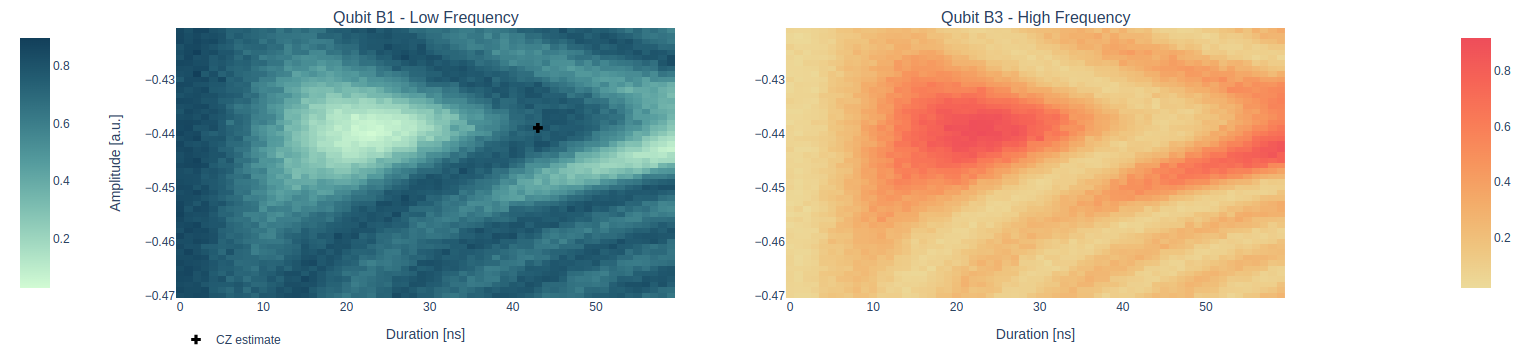
\includegraphics[width=\textwidth]{figures/png/Cryoscope/B1B3.png}
    \caption{Chevron pattern obtained from the calibration of a CZ gate on qubits \tt{B1} and \tt{B3}.}
    \label{fig:B1B3}
\end{figure}

\begin{figure}[h!]
    \centering
    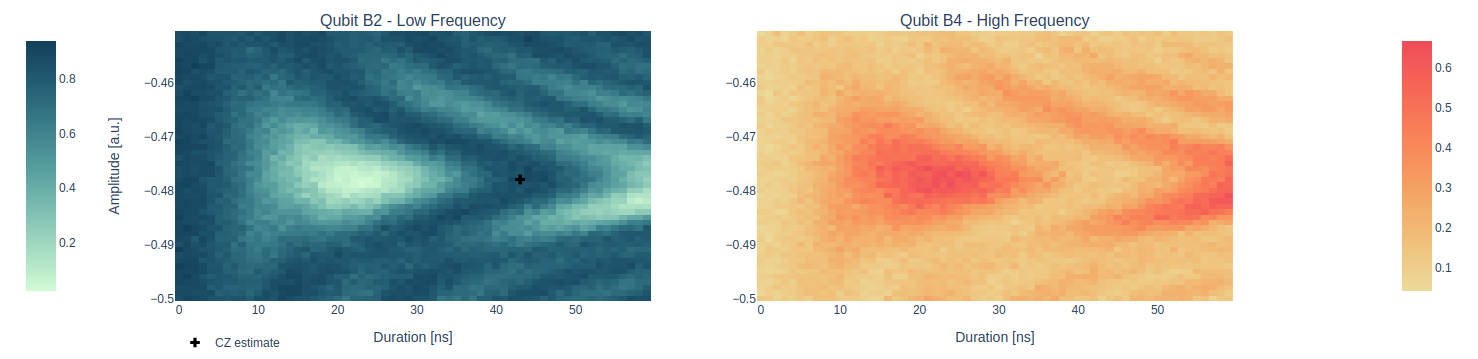
\includegraphics[width=\textwidth]{figures/png/Cryoscope/B2B4.png}
    \caption{Chevron pattern obtained from the calibration of a CZ gate on qubits \tt{B2} and \tt{B4}.}
    \label{fig:B2B4}
\end{figure}

\newpage
\restoregeometry